In this chapter, we present results in two parts. First, we show ODF templates and evaluate contrast scaling strategies for LoRE-SD. Second, we report group comparisons of fixel-wise metrics (AFD, FC, FDC) across CP, CM, and HC groups, using both MT-CSD and LoRE-SD. Key findings include increased AFD in the CP group compared to HC, particularly in the fornix and regions near the ventricles. Finally, we show that using a reduced fixel mask increases the number of significant fixels in these areas.

\section{Templates}

\begin{figure}[h!]
  \centering
  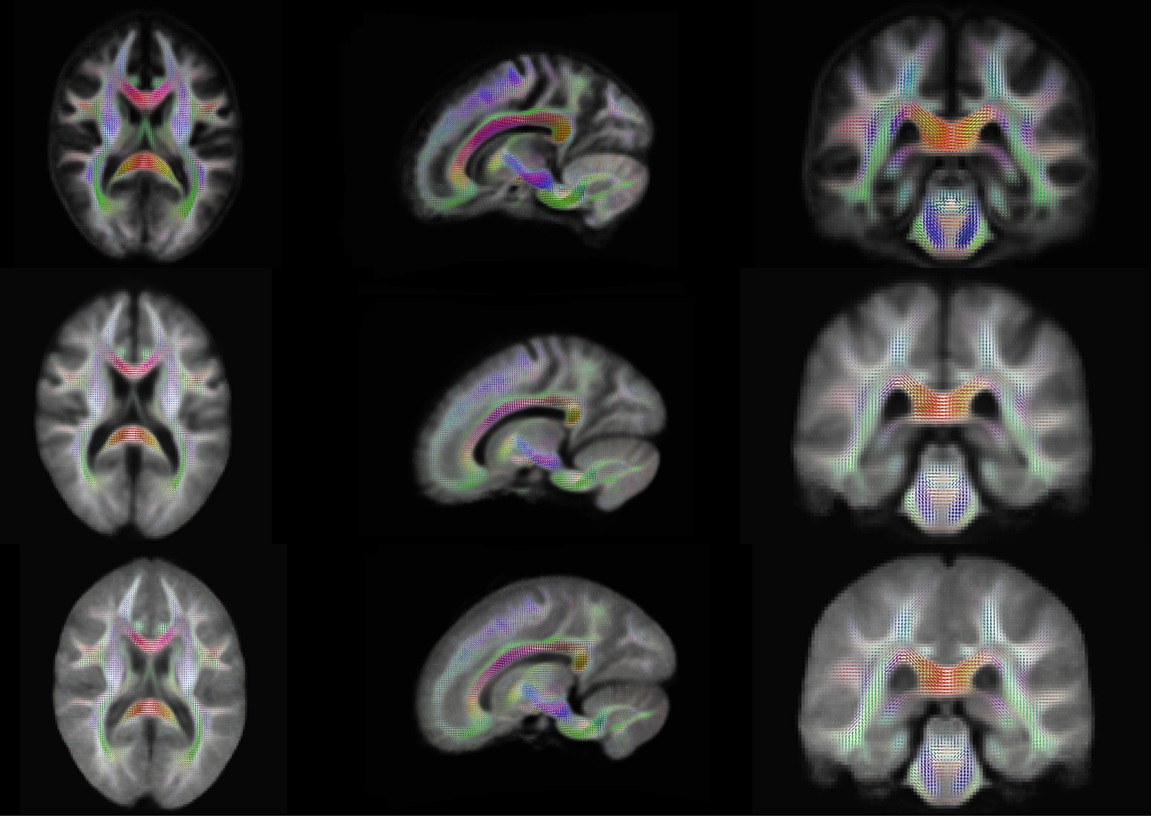
\includegraphics[width=0.8\textwidth]{Images/template_new.jpg} % or use height= for vertical sizing
  \caption{The three ODF templates used in the analysis. Top: WM ODF from MT-CSD. Middle: LoRE-SD ODF scaled with intra-axonal contrast. Bottom: LoRE-SD ODF scaled with FA contrast. ODFs are directionally colored and overlaid on a grayscale image of the first SH coefficient.}
  \label{fig:template_odf}
\end{figure}

Three ODF templates were generated and used as the basis for the subsequent analysis. An example illustrating their differences is shown in Figure~\ref{fig:template_odf}. 
\\The intra-axonal template was used as the reference space also for ODFs scaled with different contrasts (WM, FA, and anisotropic intra-axonal).


\section{LoRE-SD scaling contrasts}
\label{sec:cont}

\begin{figure}[H]
    \centering
    \subfloat[Contrast matrices.\label{fig:subfig-cont}]{
        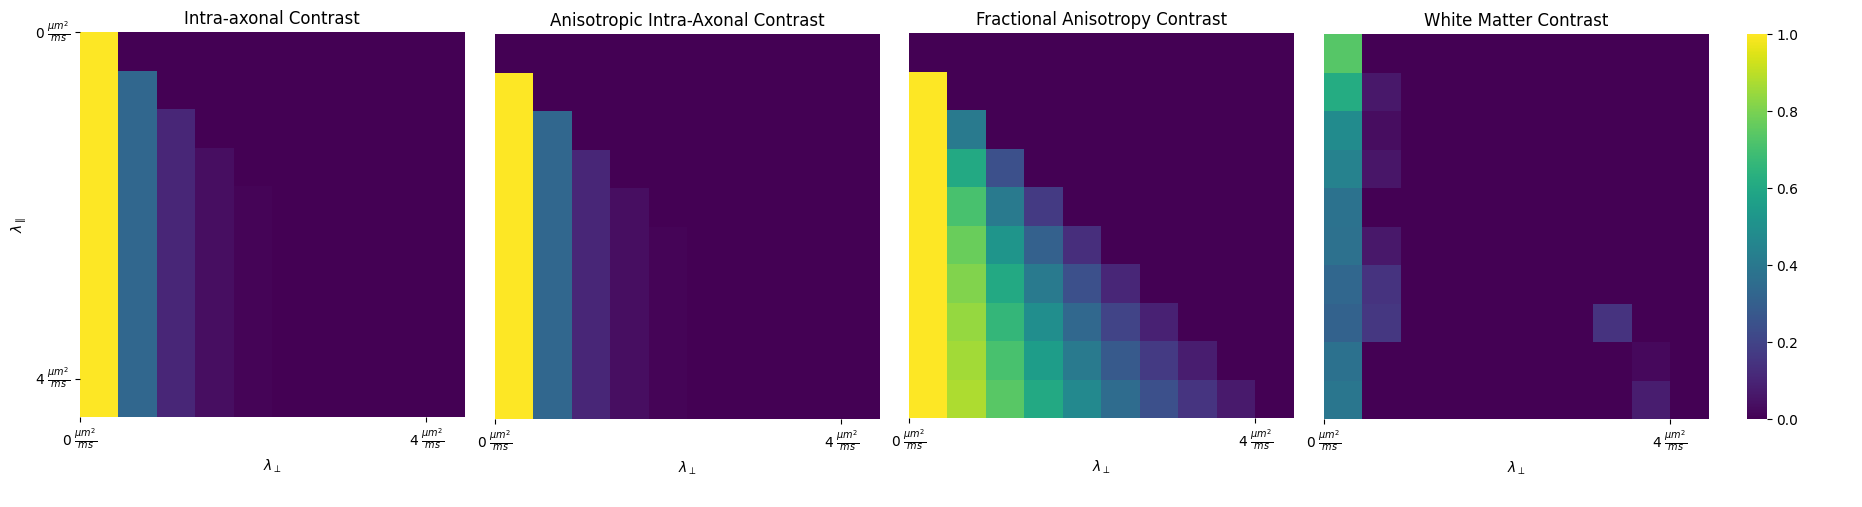
\includegraphics[width=
        \linewidth]{Images/contrast_combined.jpg}
    } \\ % <-- line break forces stacking
    \subfloat[Corresponding contrasts.\label{fig:subfig-other}]{
        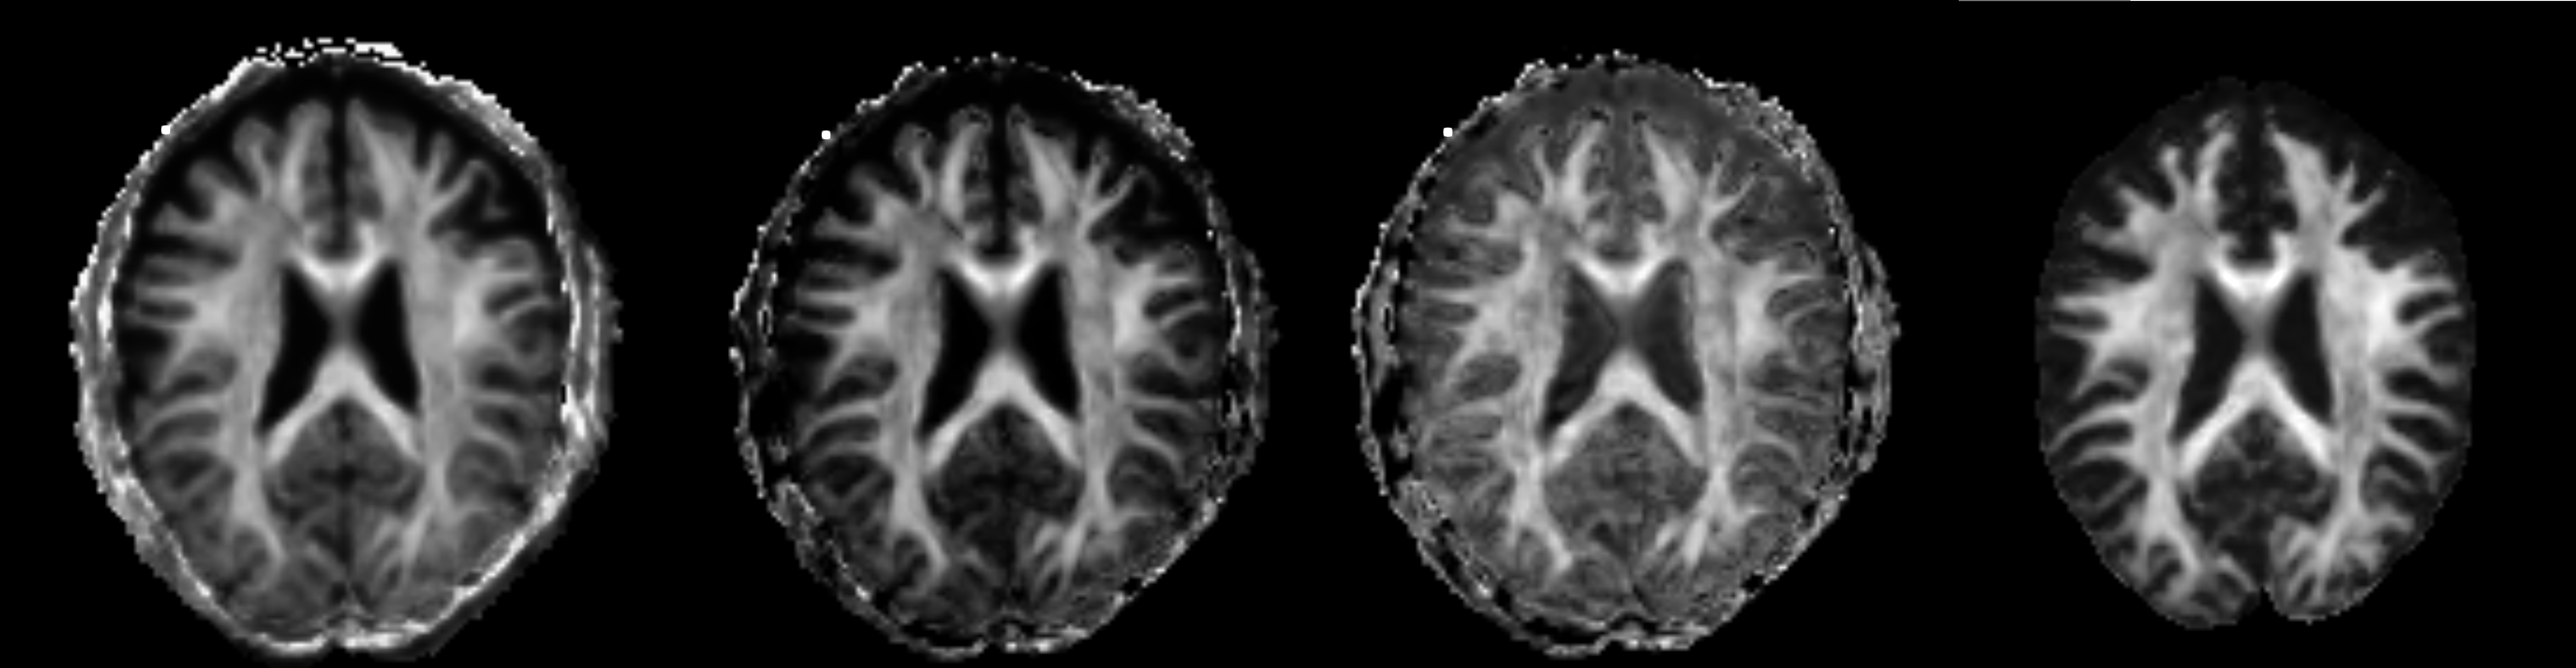
\includegraphics[width=0.8\linewidth]{Images/combined2.jpg}
    }
    \caption{Contrast matrices assigning a weight to each Gaussian basis function (a) and corresponding scaling contrasts (b) for one CP subject.}
    \label{fig:contrast_combined}
\end{figure}



Figure~\ref{fig:contrast_combined} shows all the contrast matrices and the corresponding contrasts which were used for scaling the ODFs. The fourth contrast matrix (white matter contrast) was derived for each subject by solving a constrained least squares optimization problem, aiming to find the matrix that produces a contrast best resembling the WM volume fractions obtained via MT-CSD.\\
Figure~\ref{fig:CM_10} shows the results for another subject from the CM group: the optimized contrast matrix, the resulting contrast, and the original input contrast.

For the intra-axonal contrast, making it anisotropic by setting all diagonal basis functions to zero (second matrix in ~\ref{fig:subfig-cont}) results in slightly smaller ODF amplitudes, particularly at tissue interfaces (Figure~\ref{fig:aniso}). As a consequence, fewer fixels are obtained.

\begin{figure}[h]
    \centering
    \subfloat[Contrast matrix obtained for a CM subject through optimization starting from the WM volume fractions.\label{fig:subfig-CM10}]{
        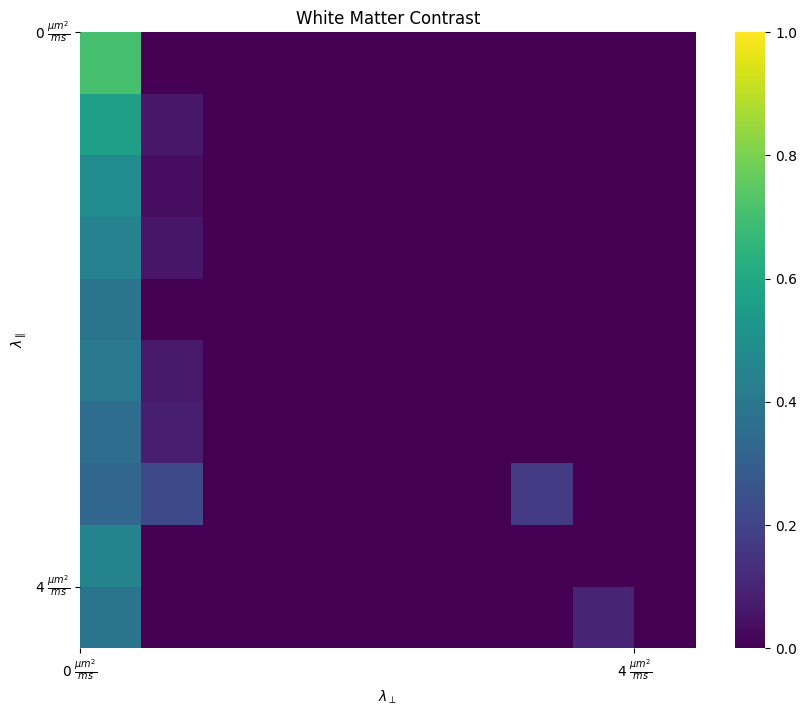
\includegraphics[width=0.5\linewidth]{Images/wm_matrix_CM_10.jpg}
    } \\[1em] % line break + vertical space
    \subfloat[Contrast obtained using the weights in a (left) and original contrast (right).\label{fig:subfig-b}]{
        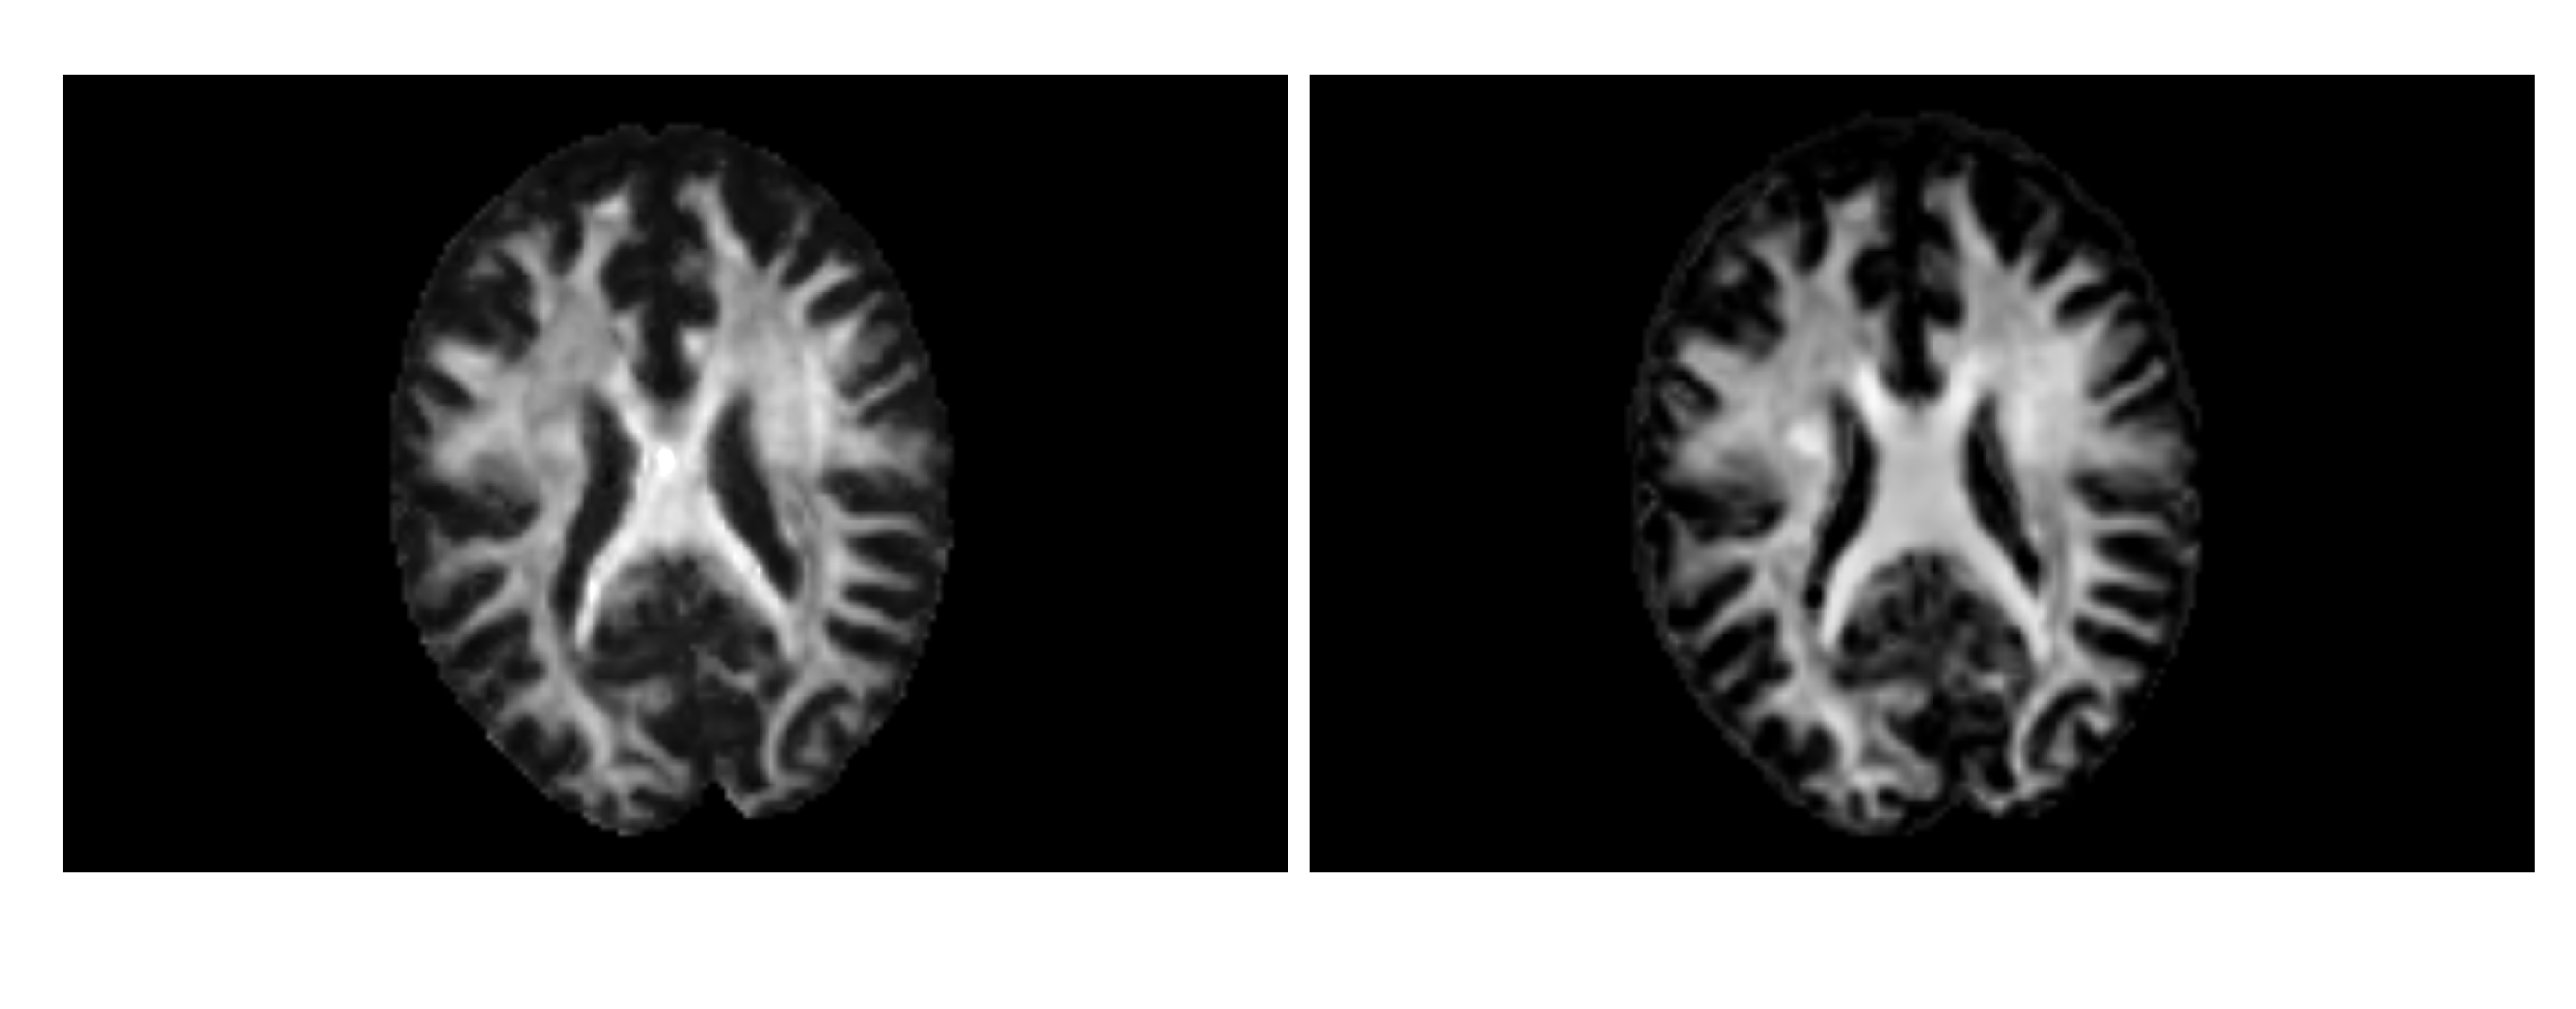
\includegraphics[width=\linewidth]{Images/CM_10.jpg}
    }
    \caption{WM contrast for a CM subject.}
    \label{fig:CM_10}
\end{figure}




\begin{figure}[H]
  \centering
  \includegraphics[width=0.9\textwidth]{Images/aniso.jpg} % or use height= for vertical sizing
  \caption{ODFs scaled with the intra-axonal contrast (left) and with the anisotropic intra-axonal contrast (right). ODFs are overlaid on a grayscale image representing the first SH coefficient.  The results are different mostly at tissue interfaces.}
  \label{fig:aniso}
\end{figure}

\section{Chemobrain}
Statistical tests were conducted to investigate differences among the CP, CM, and HC groups for the three fixel-wise metrics (AFD, log-FC, FDC), initially analyzing the whole brain excluding only the brainstem and cerebellum. Significant regions were identified as those containing fixels with a FWE-corrected p-value below 5\%. In this section, figures displaying results show fixels overlaid on grayscale images representing the first SH coefficient of the corresponding ODF template. This way anatomical context is provided. 

\subsection{MSMT-CSD}
Significant results were found for AFD when testing for a higher value in the CP group compared to HC. We found 637 significant fixels. No significant differences were found in any case for FDC and FC. 
\\AFD was significantly higher for fixels belonging to the fornix (Figure~\ref{fig:fornix1} and \ref{fig:fornix2}), but also in regions at the interface with the ventricles (Figure~\ref{fig:inter}) and in crossing fibre regions (Figure~\ref{fig:cross}).

\begin{figure}[h]
  \centering
  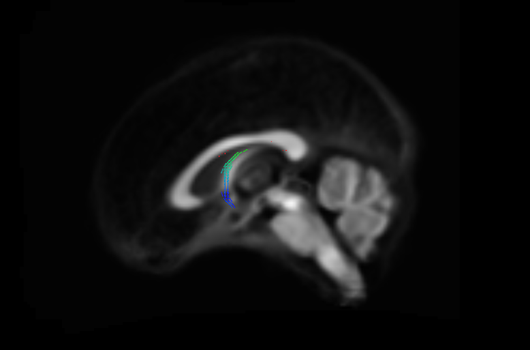
\includegraphics[width=0.9\textwidth]{Images/fornix1.jpg} % or use height= for vertical sizing
  \caption{Fixels derived with MT-CSD. Significant fixels found when testing a higher AFD in CP compared to HC. Significant fixels are colored based on their direction. The sagittal slice clearly shows the fornix as a region with significant AFD increase.}
  \label{fig:fornix1}
\end{figure}

\begin{figure}[H]
  \centering
  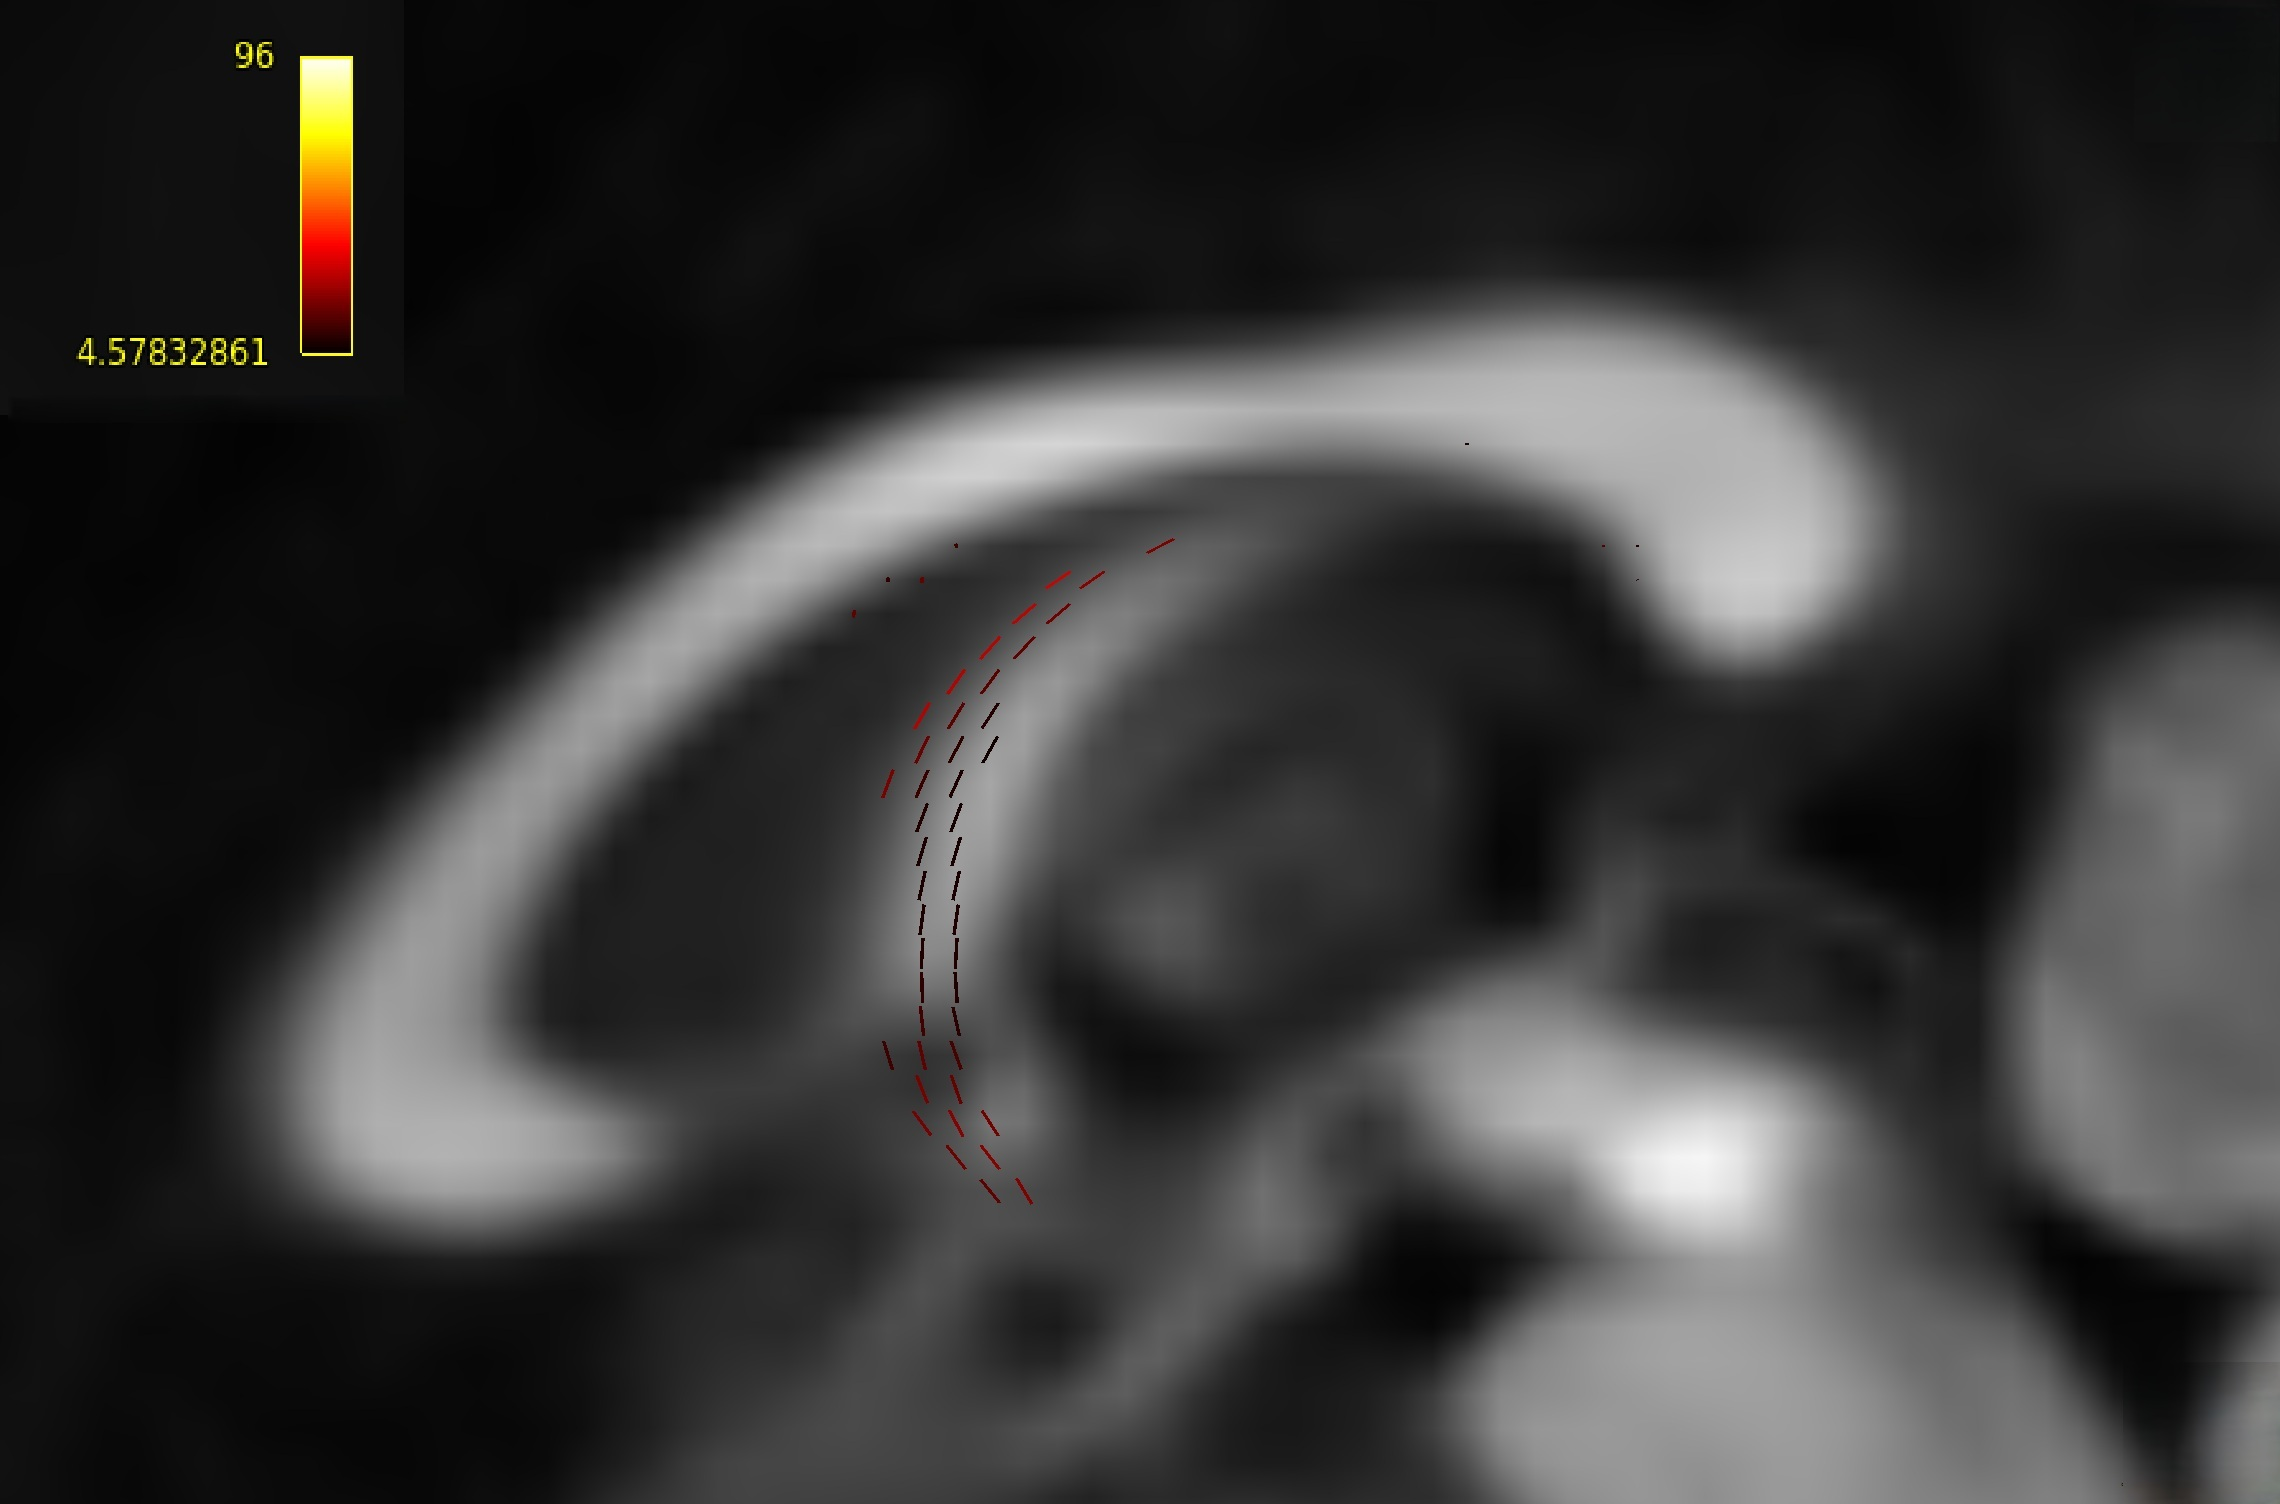
\includegraphics[width=0.8\textwidth]{Images/fornix2.jpg} % or use height= for vertical sizing
  \caption{Fixels derived with MT-CSD. Significant fixels found when testing for higher AFD in the CP group compared to HC. The image shows a zoomed-in view of the fornix, with significant fixels colored by the percentage increase in AFD relative to the average value in the HC group. Since AFD is a relative measure with arbitrary units, the absolute effect size (the difference in mean AFD between groups) is converted to percentage of the HC mean. The increase in the fornix remains small.}
  \label{fig:fornix2}
\end{figure}


\begin{figure}[H]
  \centering
  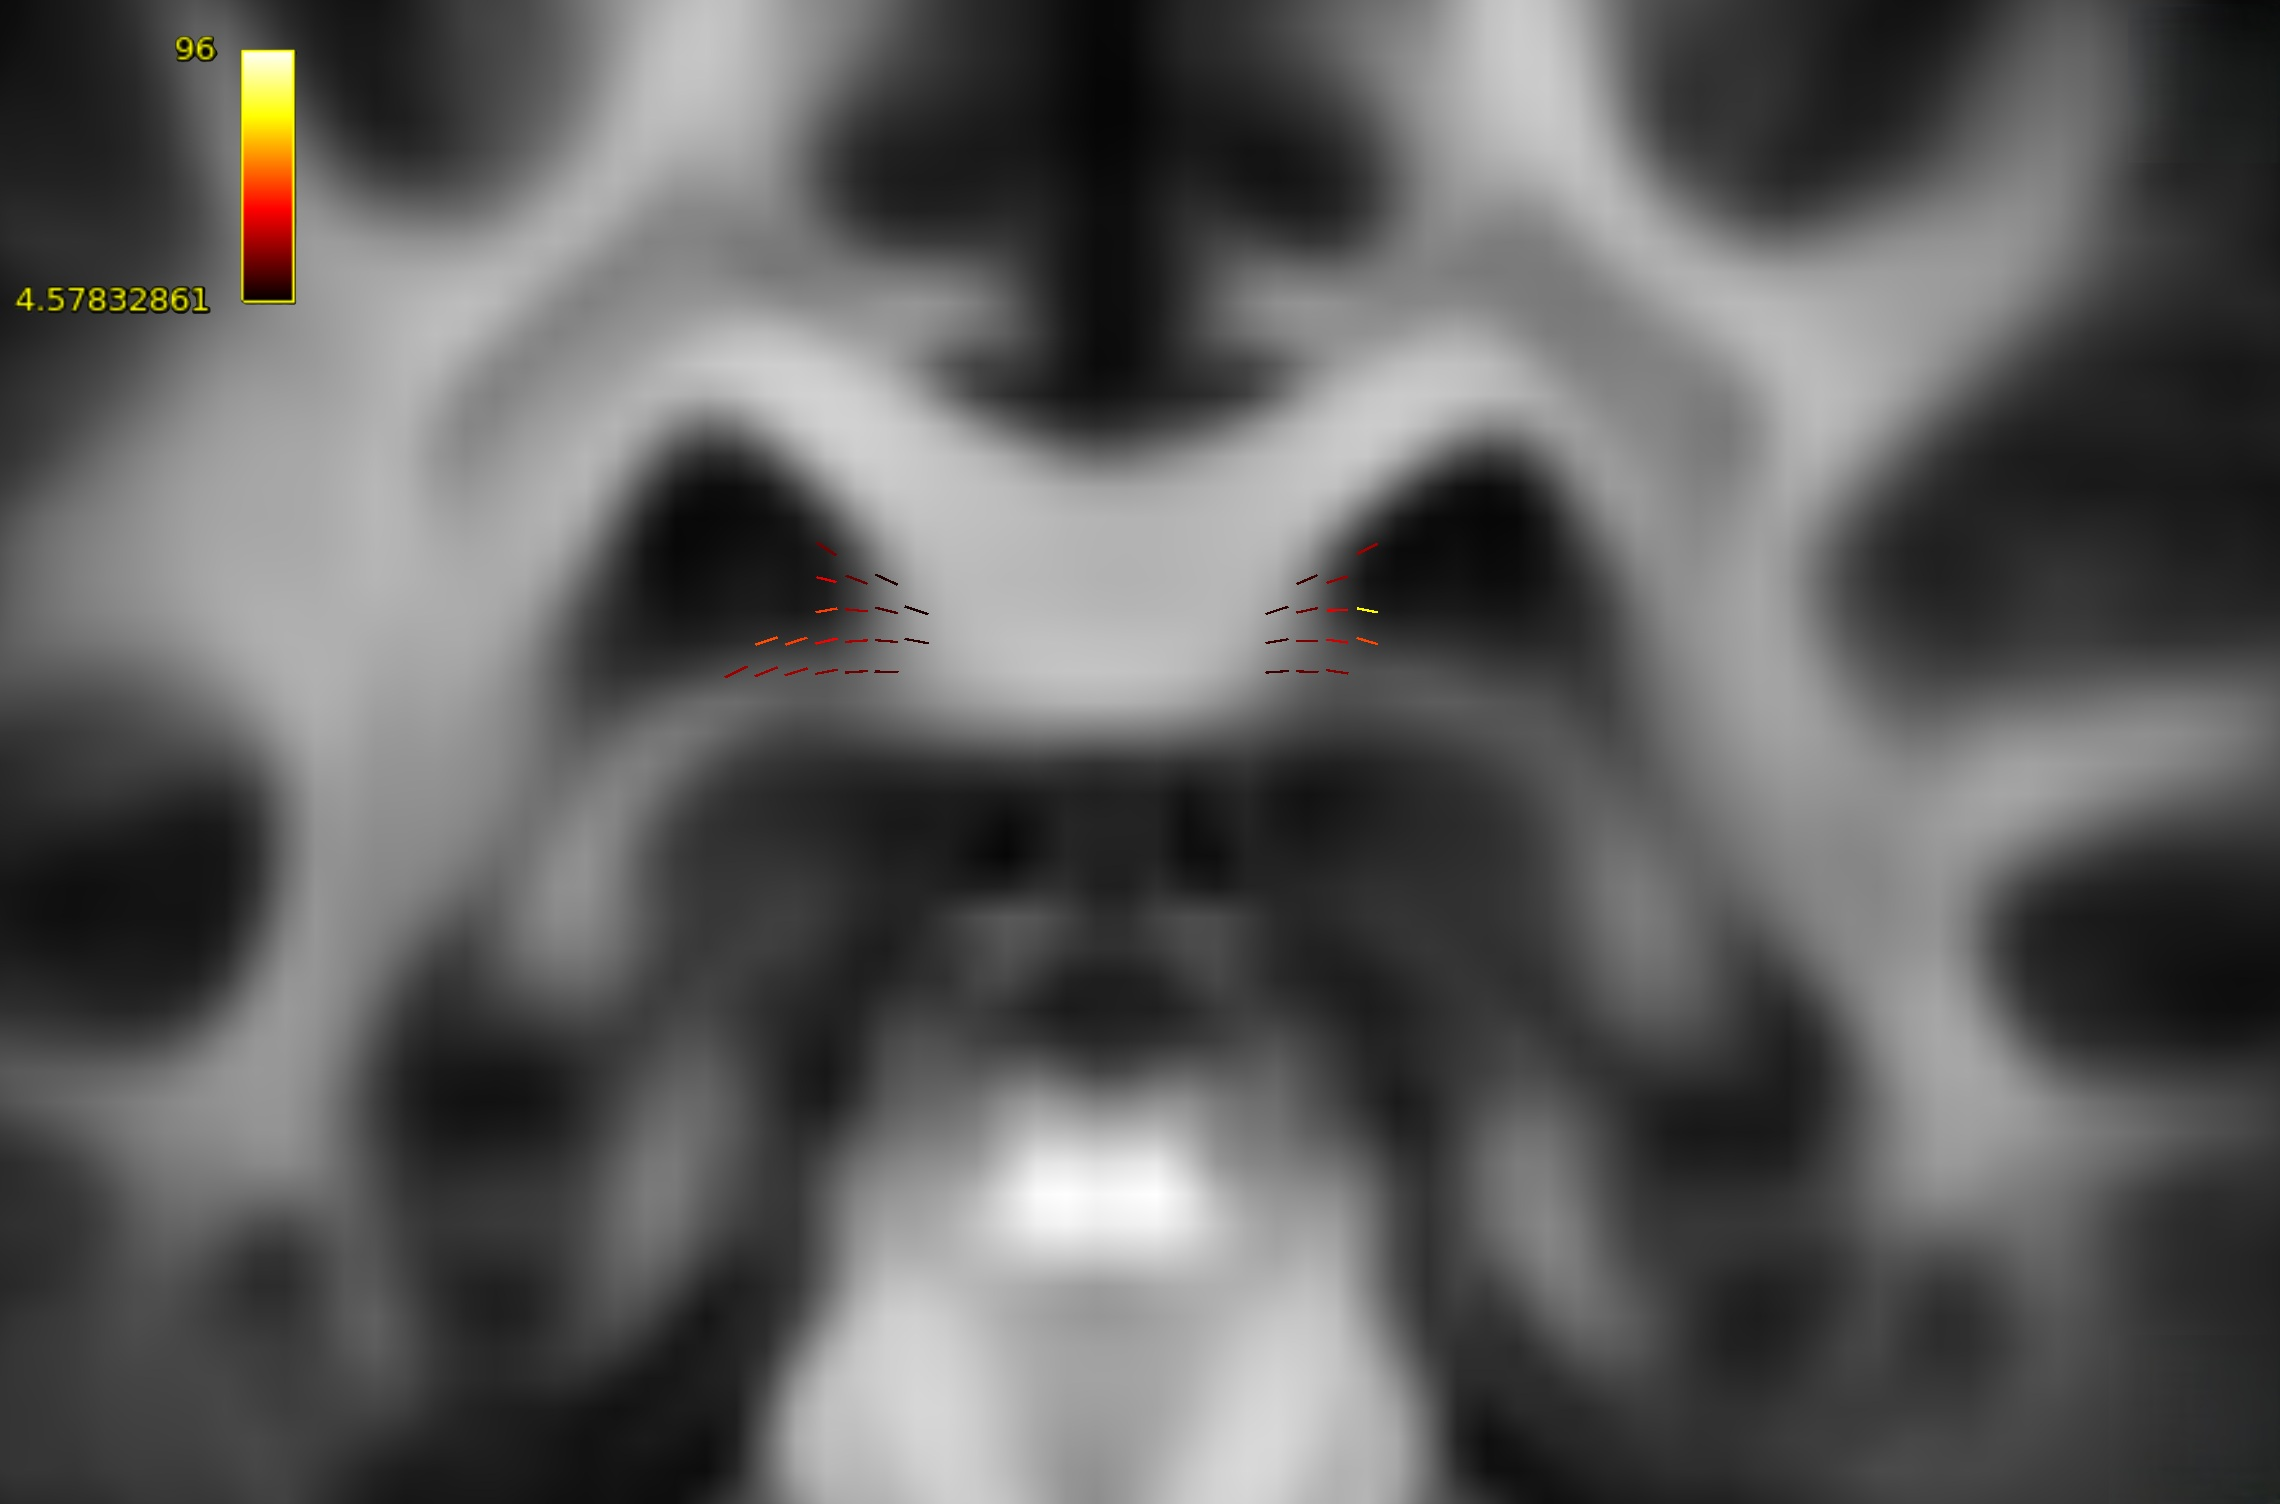
\includegraphics[width=0.8\textwidth]{Images/inter.jpg} % or use height= for vertical sizing
  \caption{Fixels derived with MT-CSD. Significant fixels found when testing for higher AFD in the CP group compared to HC. Detail showing significant fixels at the interface between the corpus callosum and the ventricles, colored by percentage increase in AFD relative to the HC mean. The effect size is larger in regions closer to the ventricles.}
  \label{fig:inter}
\end{figure}

\begin{figure}[H]
    \centering
    \subfloat[Fixels derived with MT-CSD. Results of testing for higher AFD in the CP group compared to HC.]{
        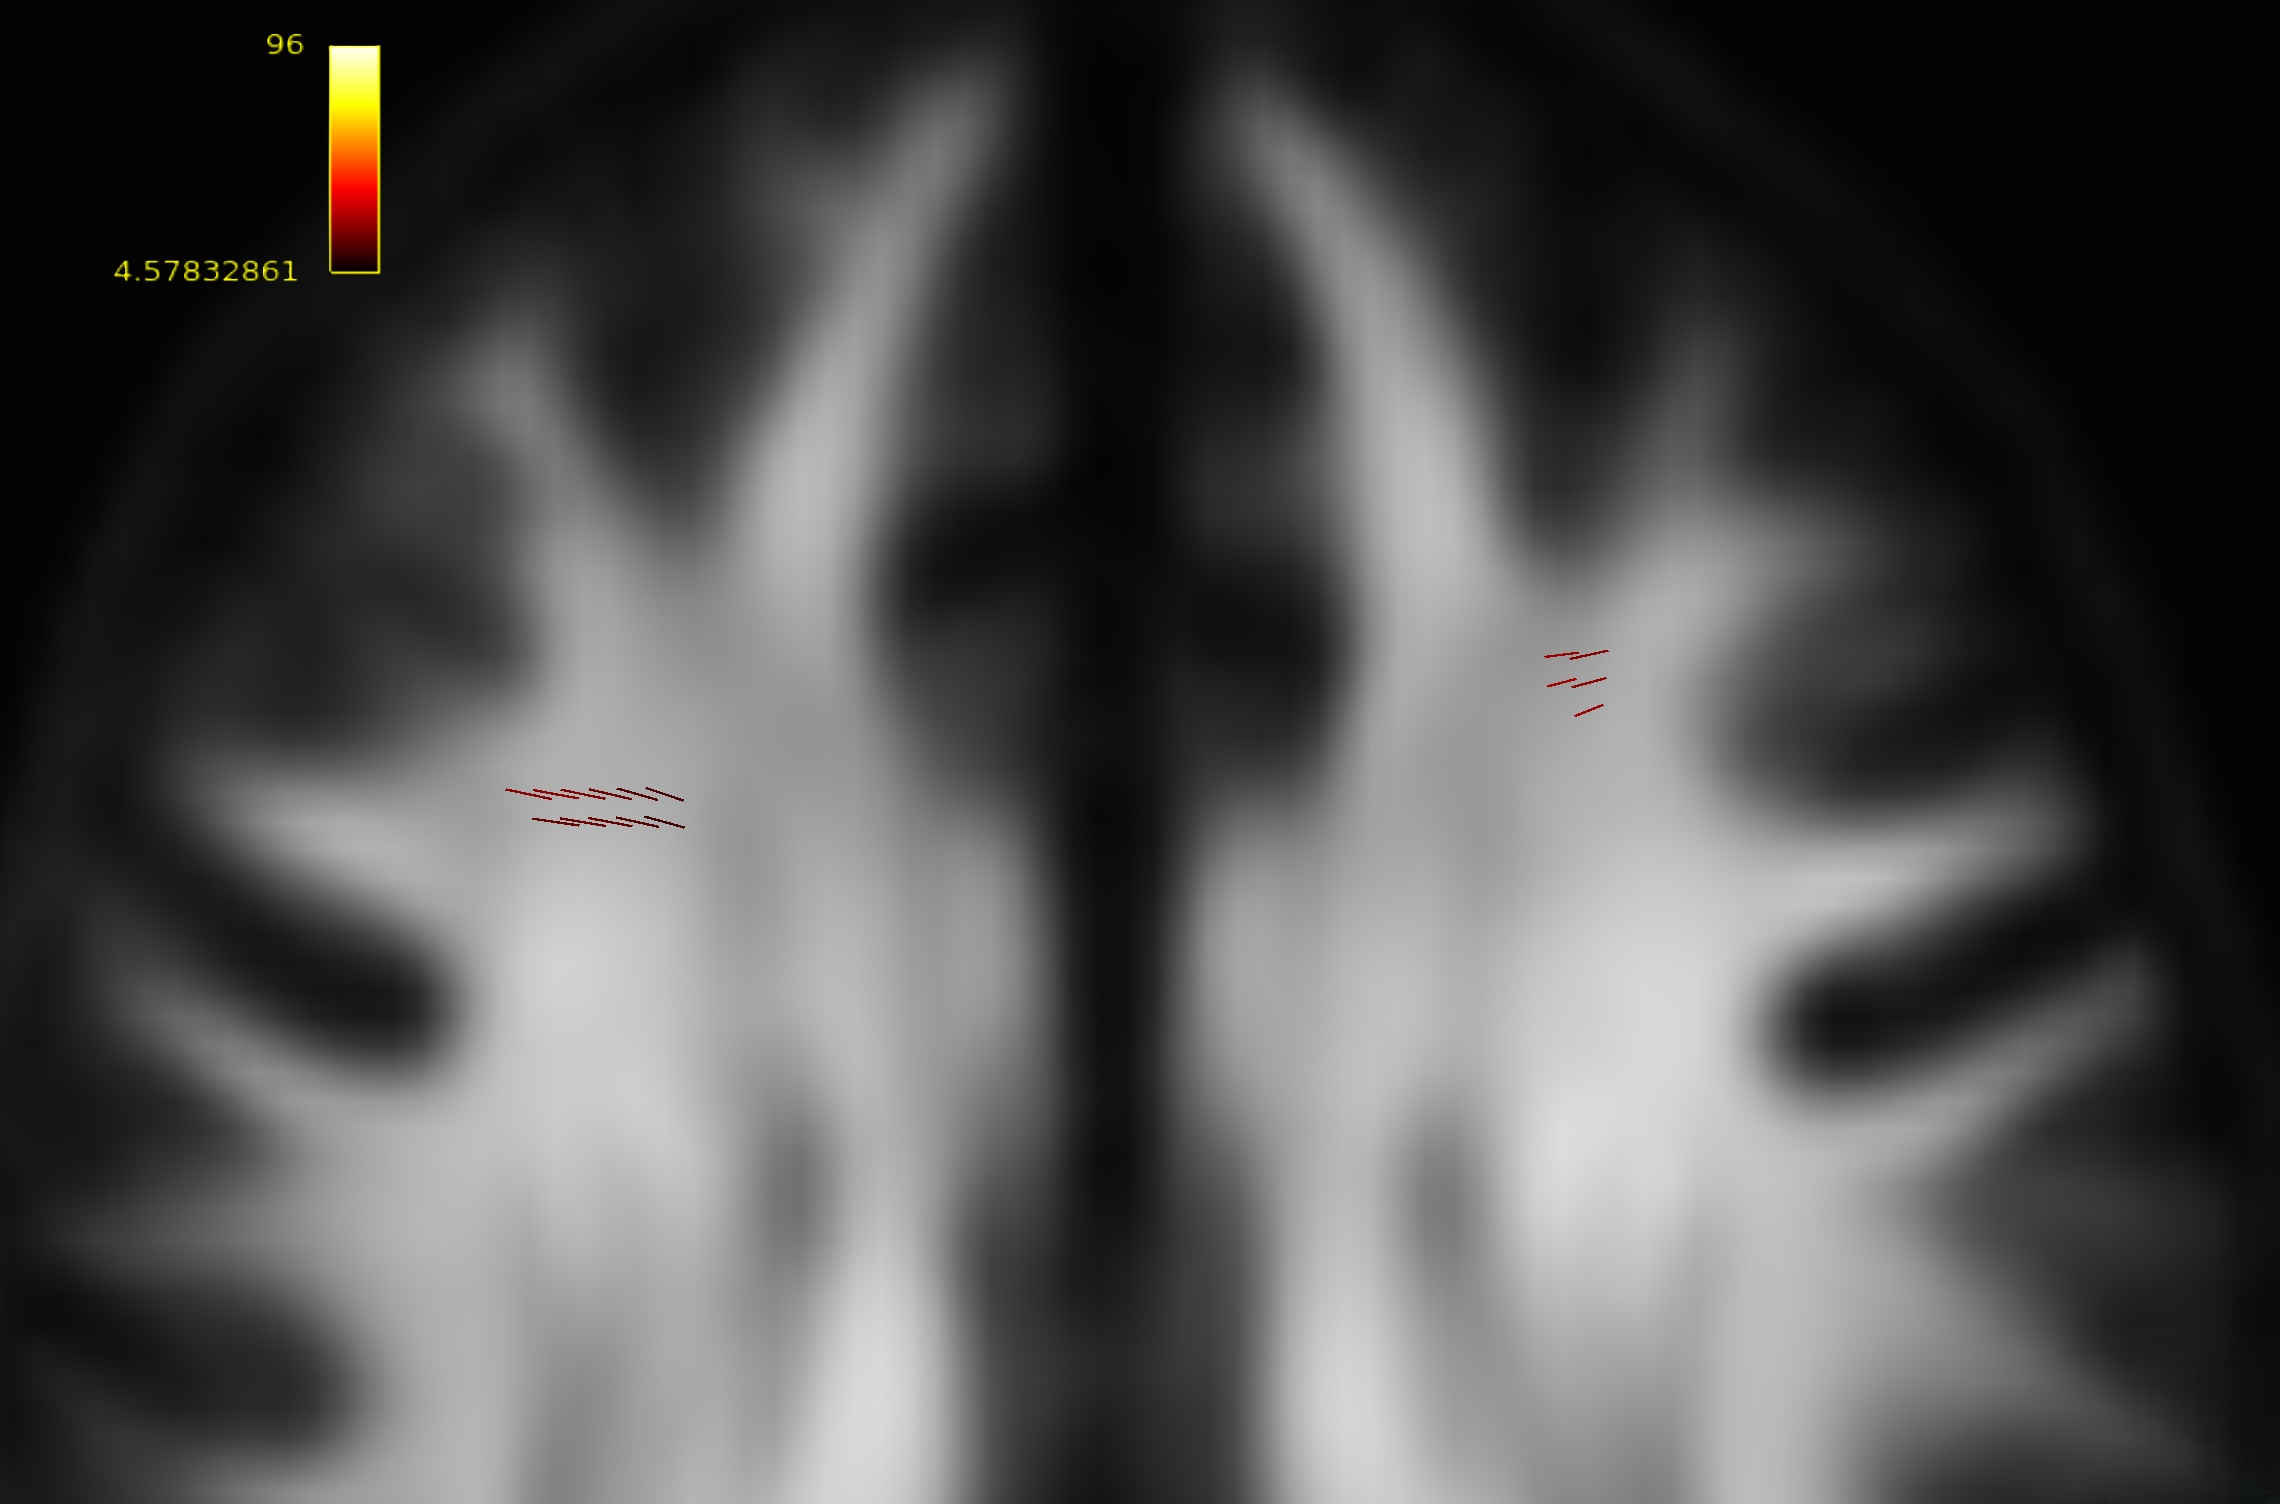
\includegraphics[width=0.45\linewidth]{Images/cross1.jpg}
    \label{fig:subfig-cross1}}
    \hfill
    \subfloat[All fixels included in the fixel mask for the MT-CSD template. Red circles show regions of interest.]{
        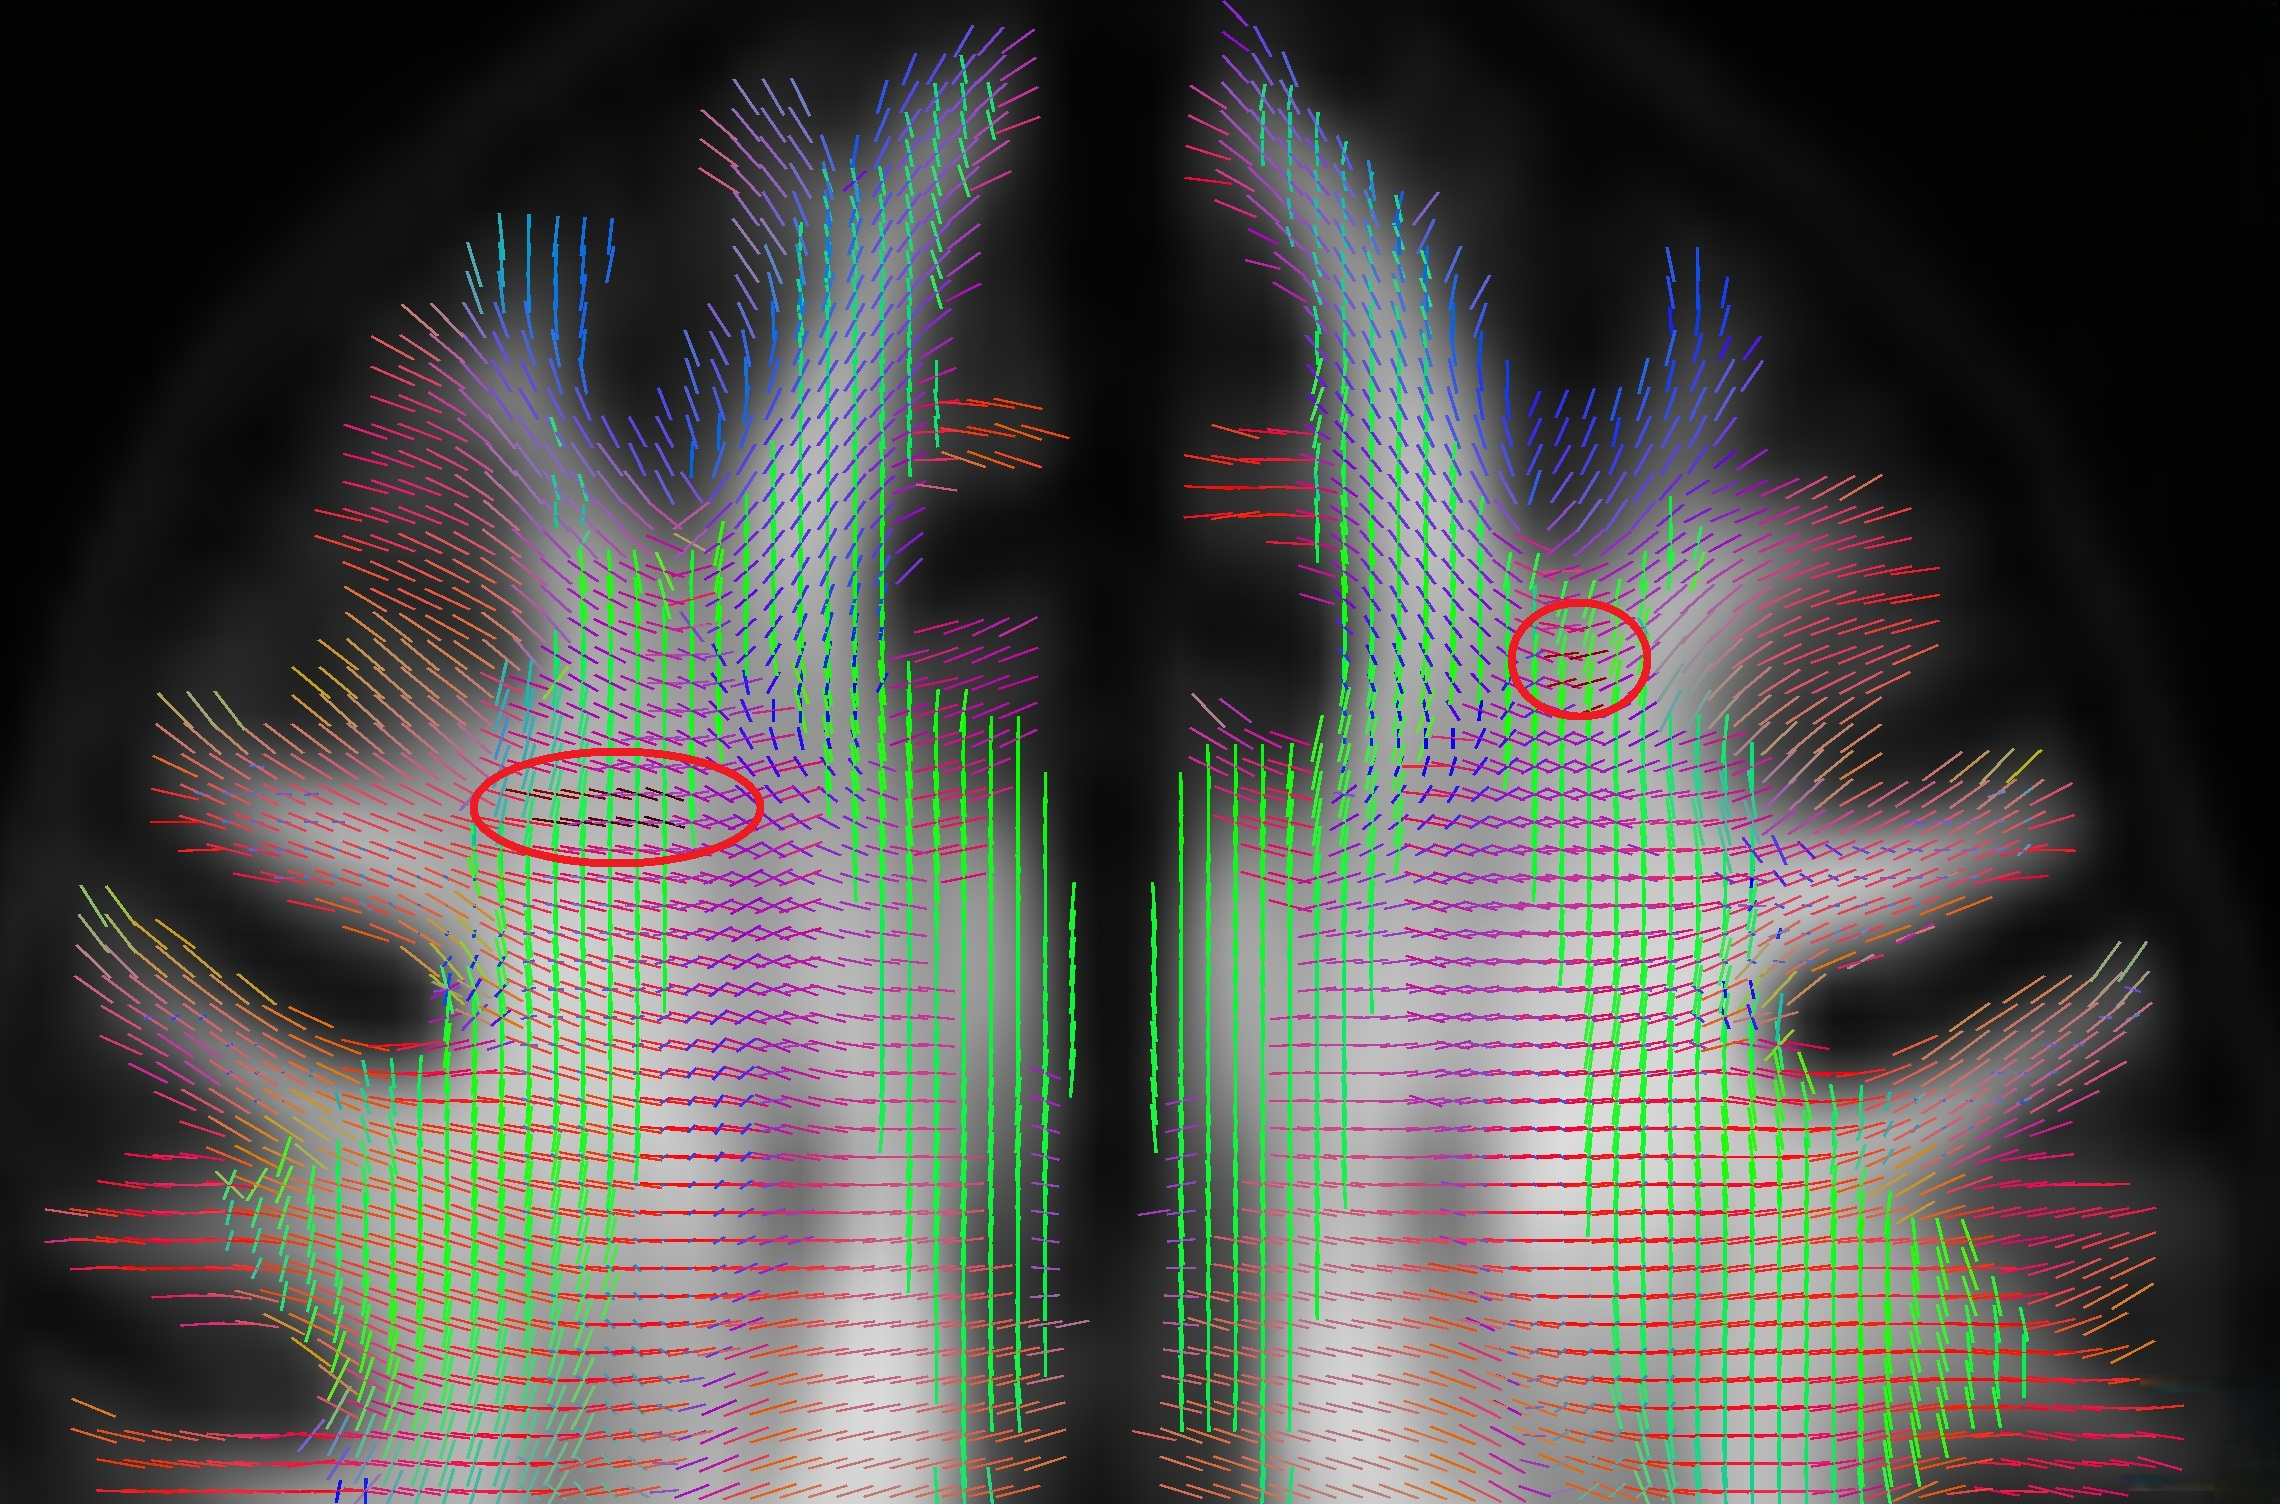
\includegraphics[width=0.45\linewidth]{Images/cross2.jpg}
    \label{fig:subfig-cross2}}
    \caption{(a) significant fixels in crossing regions, colored by percentage increase relative to HC. (b) all fixels in the mask, colored by directionality. Red circles indicate the crossing fibre regions where significant fixels were found.}
    \label{fig:cross}
\end{figure}


\subsection{LoRE-SD}
Different scaling contrasts applied to the ODFs produced varying outcomes of the statistical analysis.
When using the intra-axonal contrast for scaling, significant fixels were observed only for the AFD metric, and exclusively when testing for an increase in CP compared to HC. A total of 16 significant fixels were identified. No significant fixels were found for the other two metrics. The significant fixels and a comparison with the results when using MT-CSD in the same region  are shown in Figure~\ref{fig:Lore_comp}. 


\begin{figure}[h]
    \centering
    \subfloat[LoRE-SD with intra-axonal scaling]{
        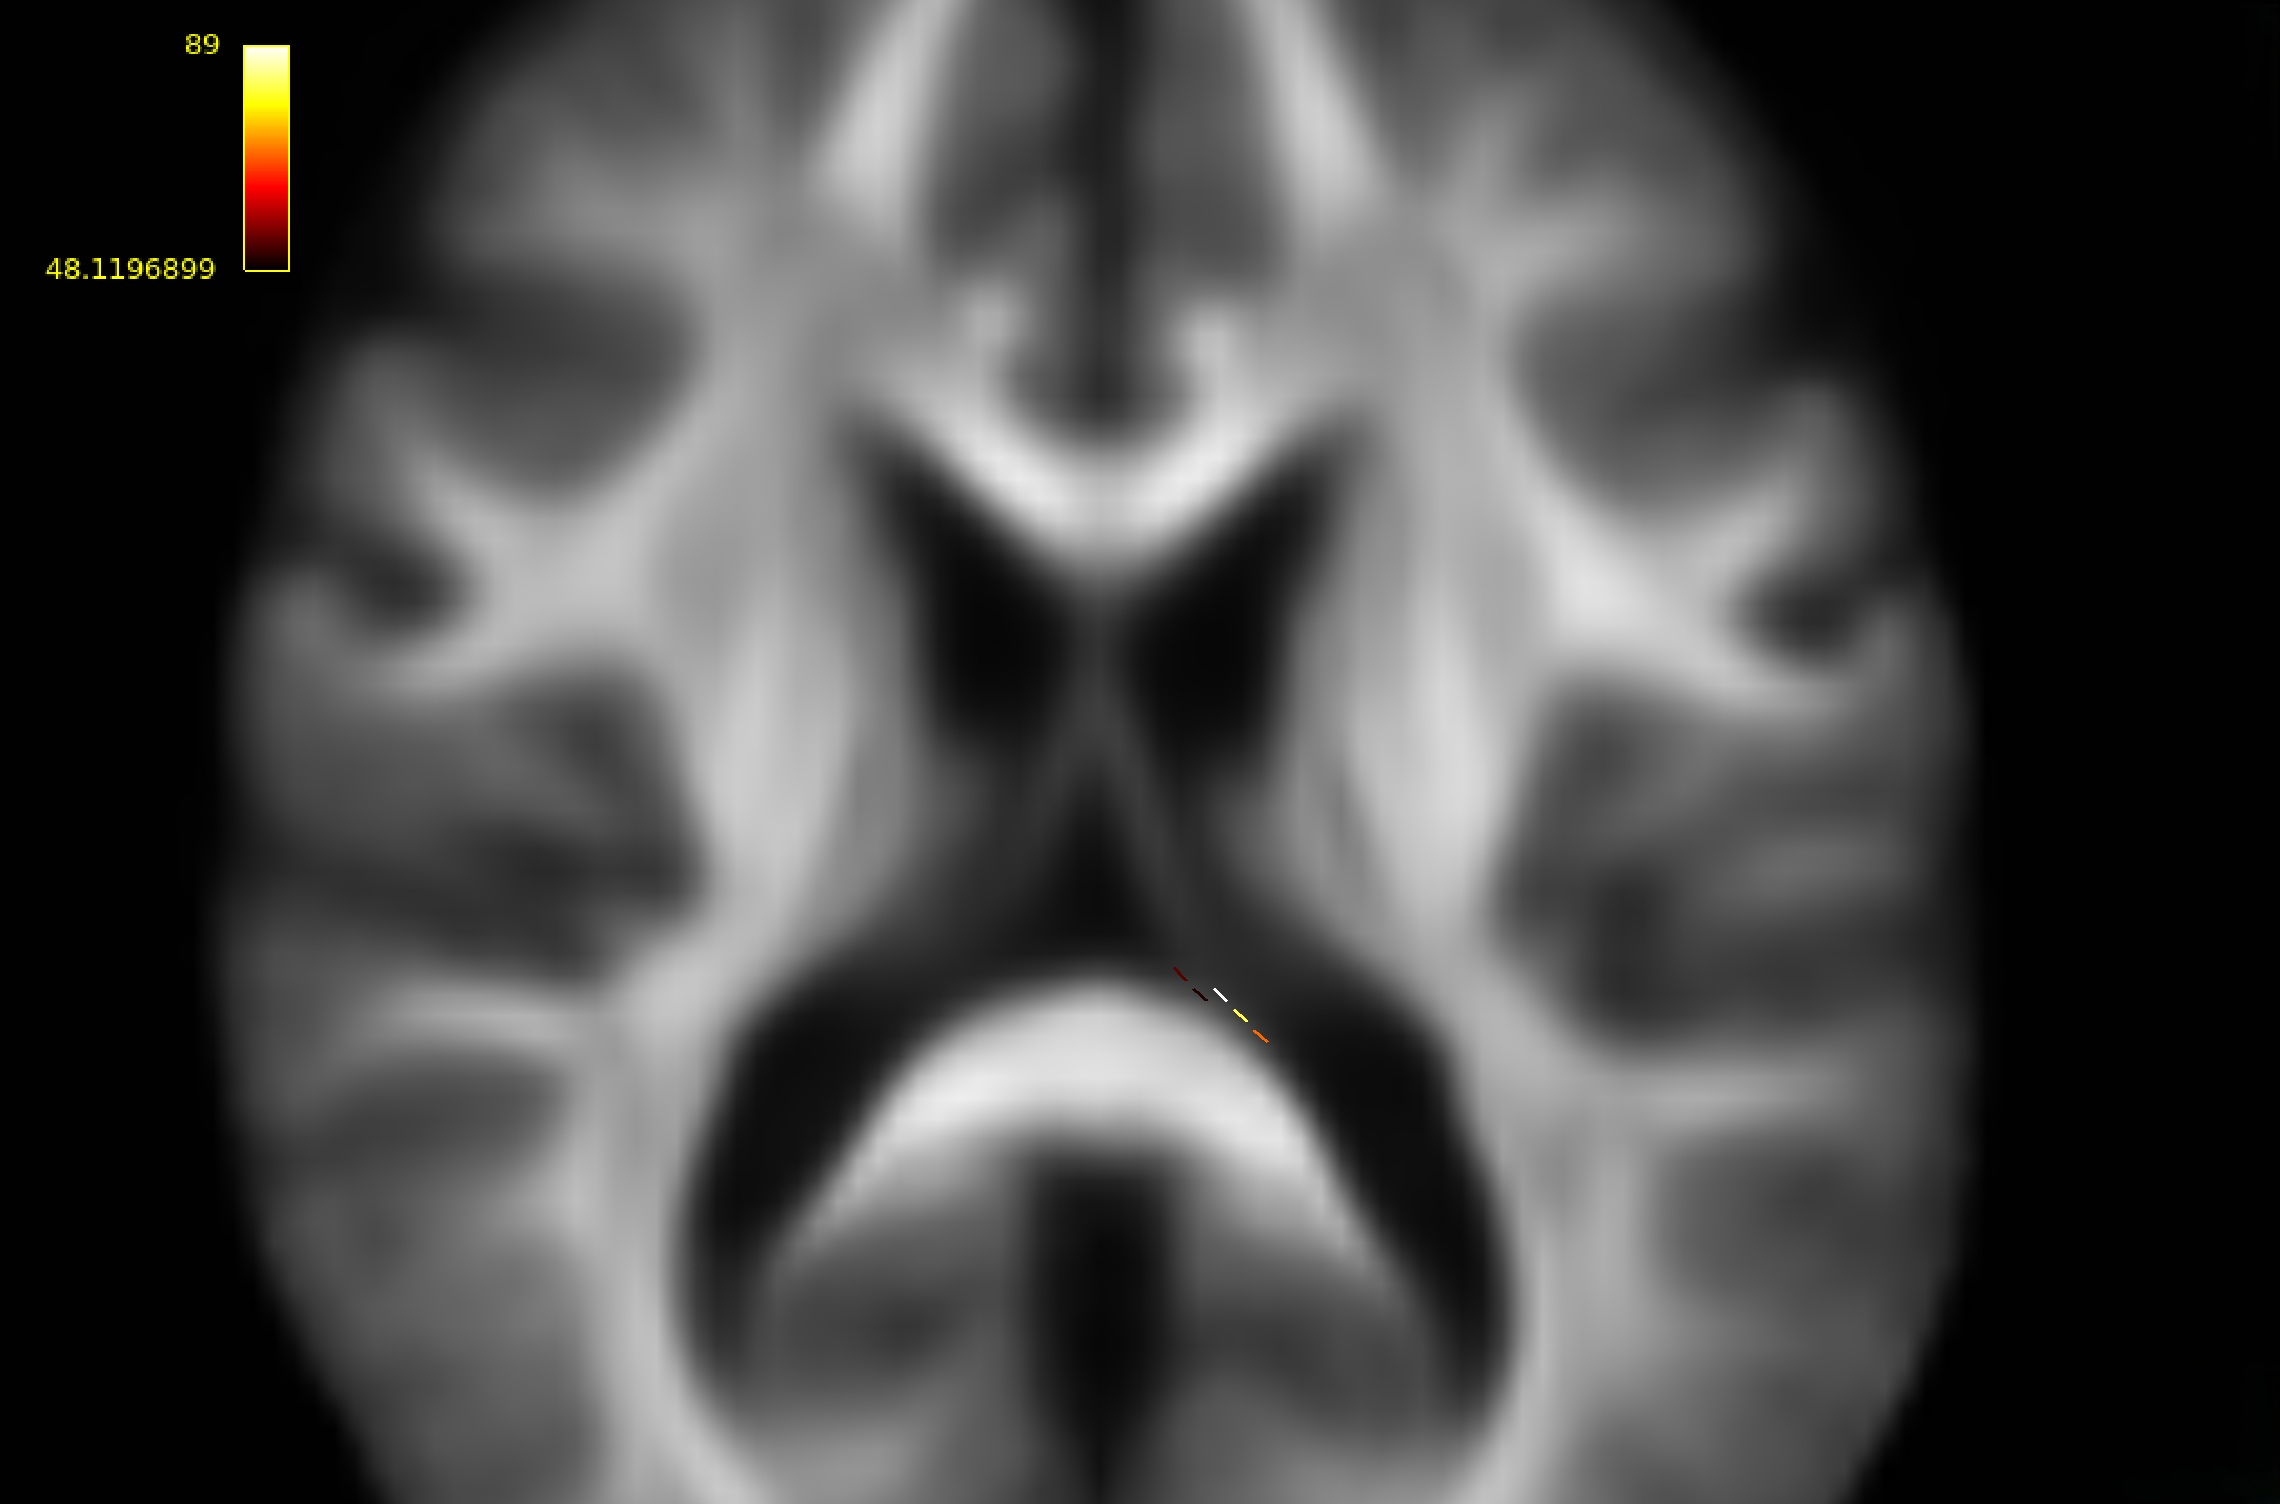
\includegraphics[width=0.45\linewidth]{Images/comp_final_intra.jpg}
        \label{fig:subfig-lore-intra}
    }
    \hfill
    \subfloat[MT-CSD]{
        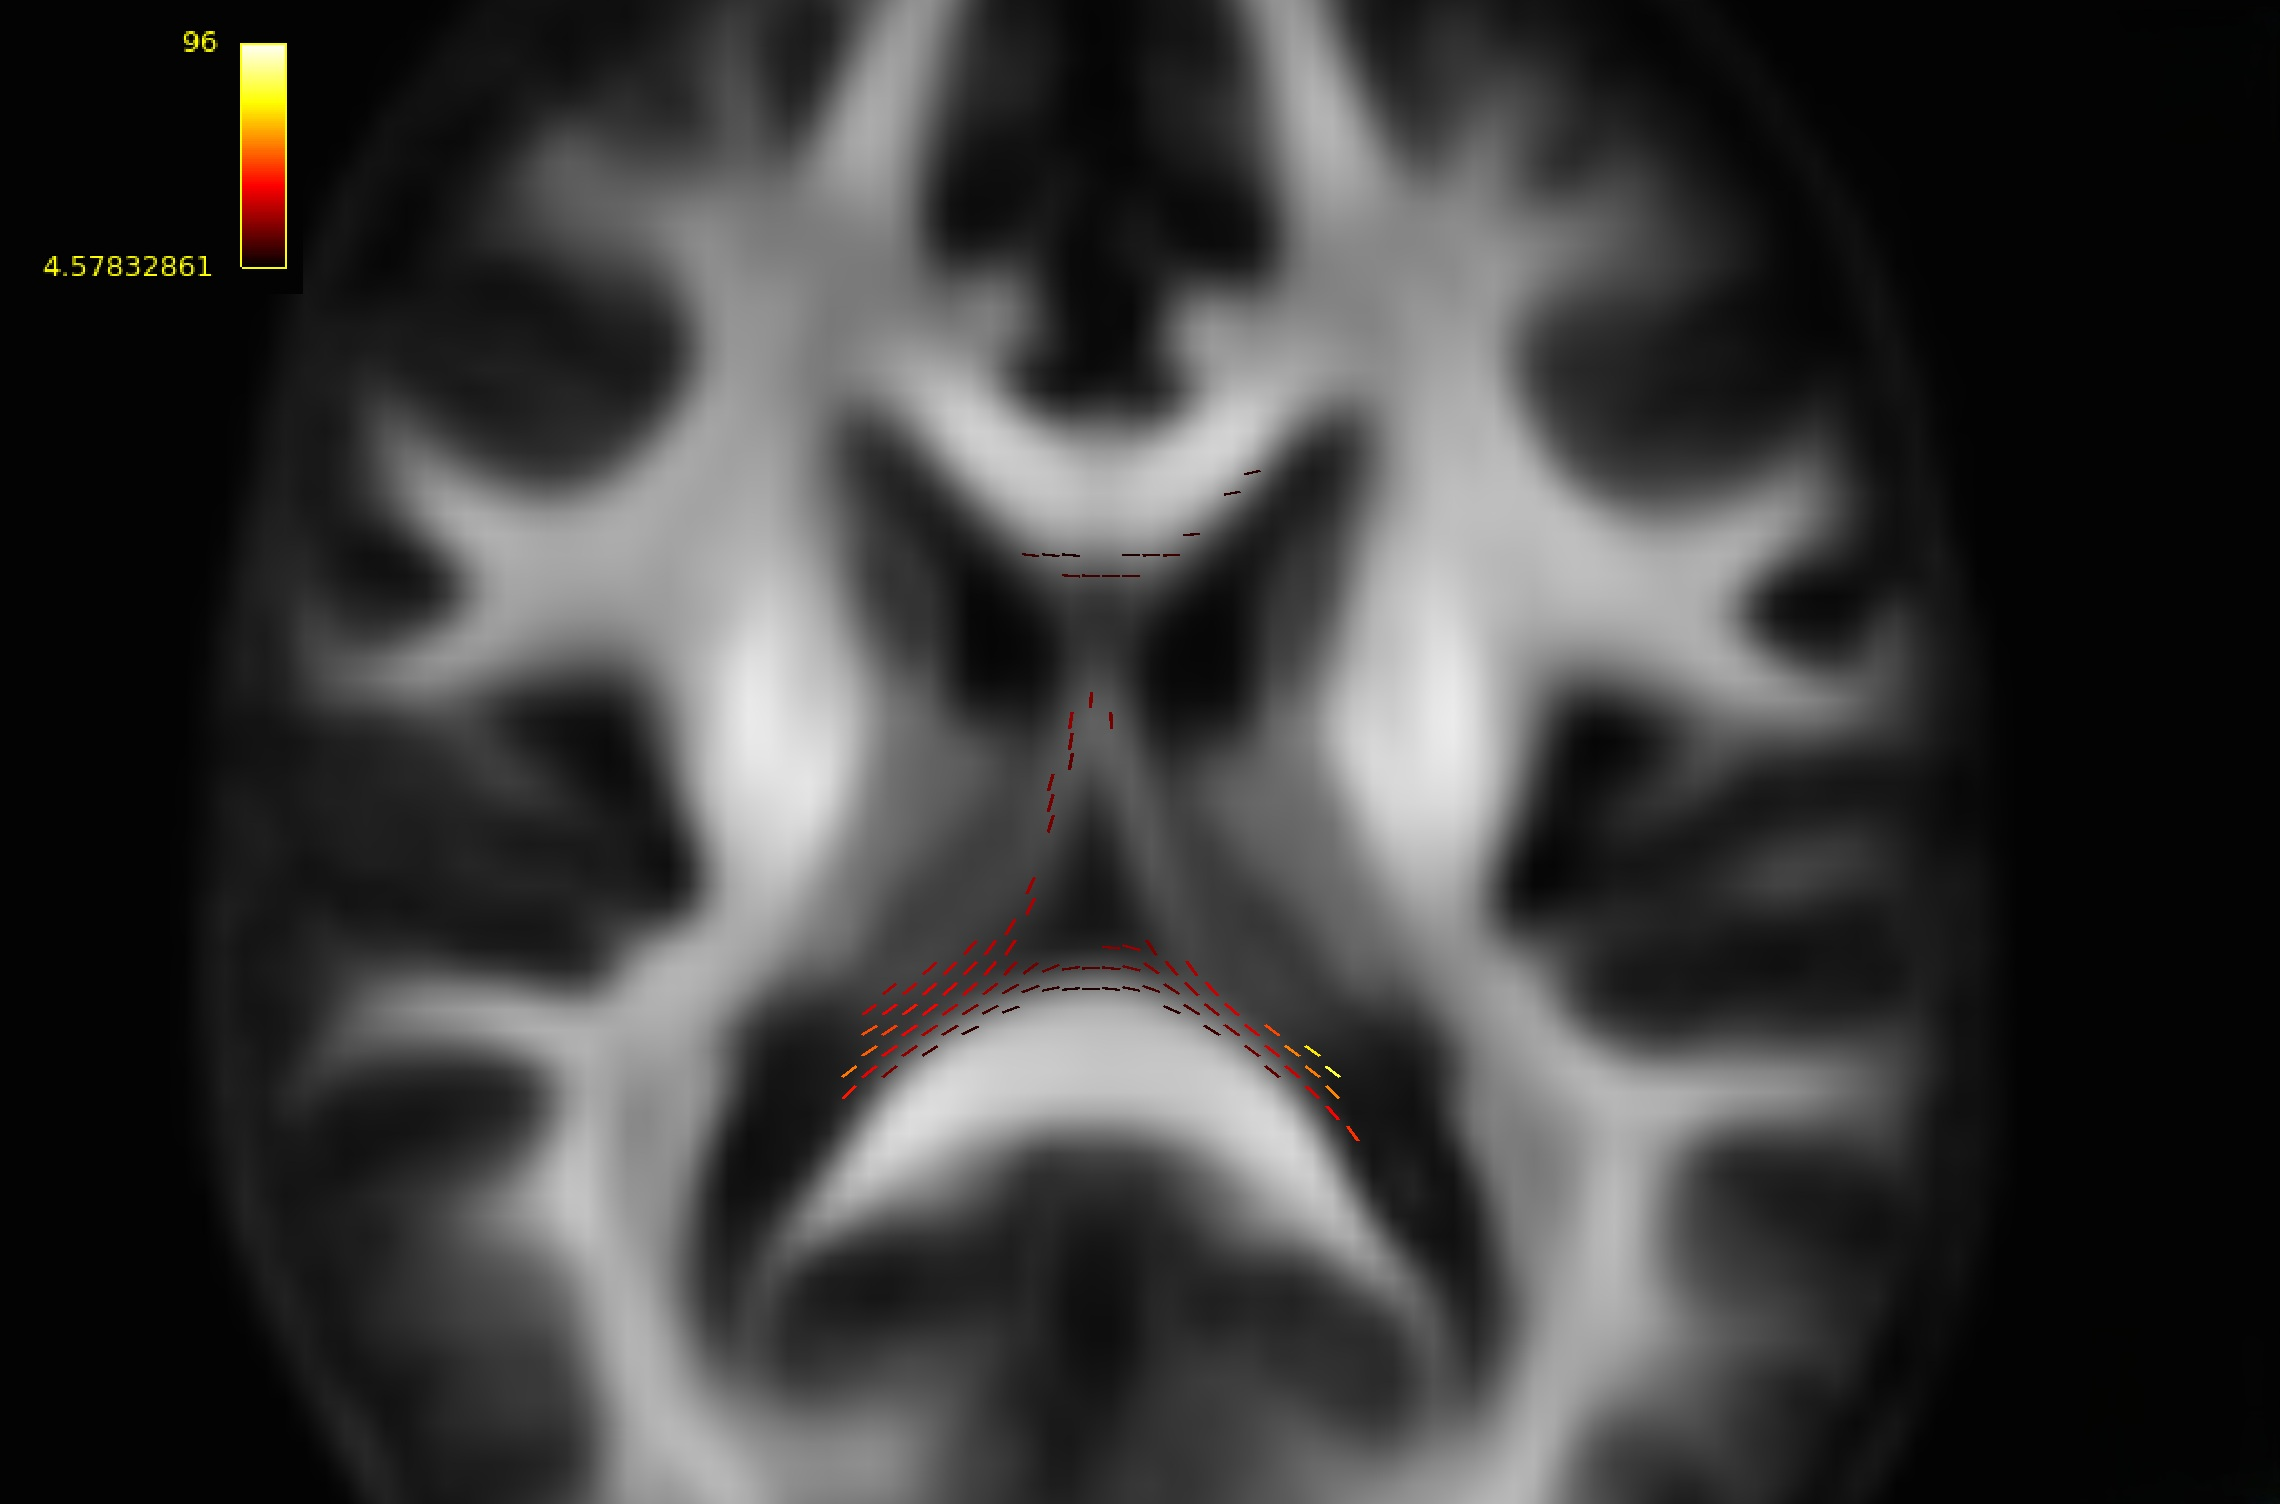
\includegraphics[width=0.45\linewidth]{Images/comp_final_MT.jpg}
        \label{fig:subfig-mtcsd}
    }
    \caption{Left: LoRE-SD scaled with the intra-axonal contrast, testing for higher AFD in CP compared to HC. The fixels highlight a region at the interface with the ventricles. Right: significant fixels in the same area for MT-CSD for the same test, including fixels in the fornix and CC.}
    \label{fig:Lore_comp}
\end{figure}


With the FA and the anisotropic-intra-axonal contrast no significant results were found. Finally for the WM contrast we found a significant increase of AFD in CP compared to HC. Only 78 fixels were found to be significant. Similarly to MT-CSD, the fixels were part of the fornix and at the tissue interface with the ventricles, but no significance was found in the crossing fibre regions. Significant results are in Figure~\ref{fig:fornix4} and ~\ref{fig:wm_result}. No differences where found for the other group comparisons or for the other two metrics.


\begin{figure}[H]
    \centering
    \subfloat[Sagittal view.]{
        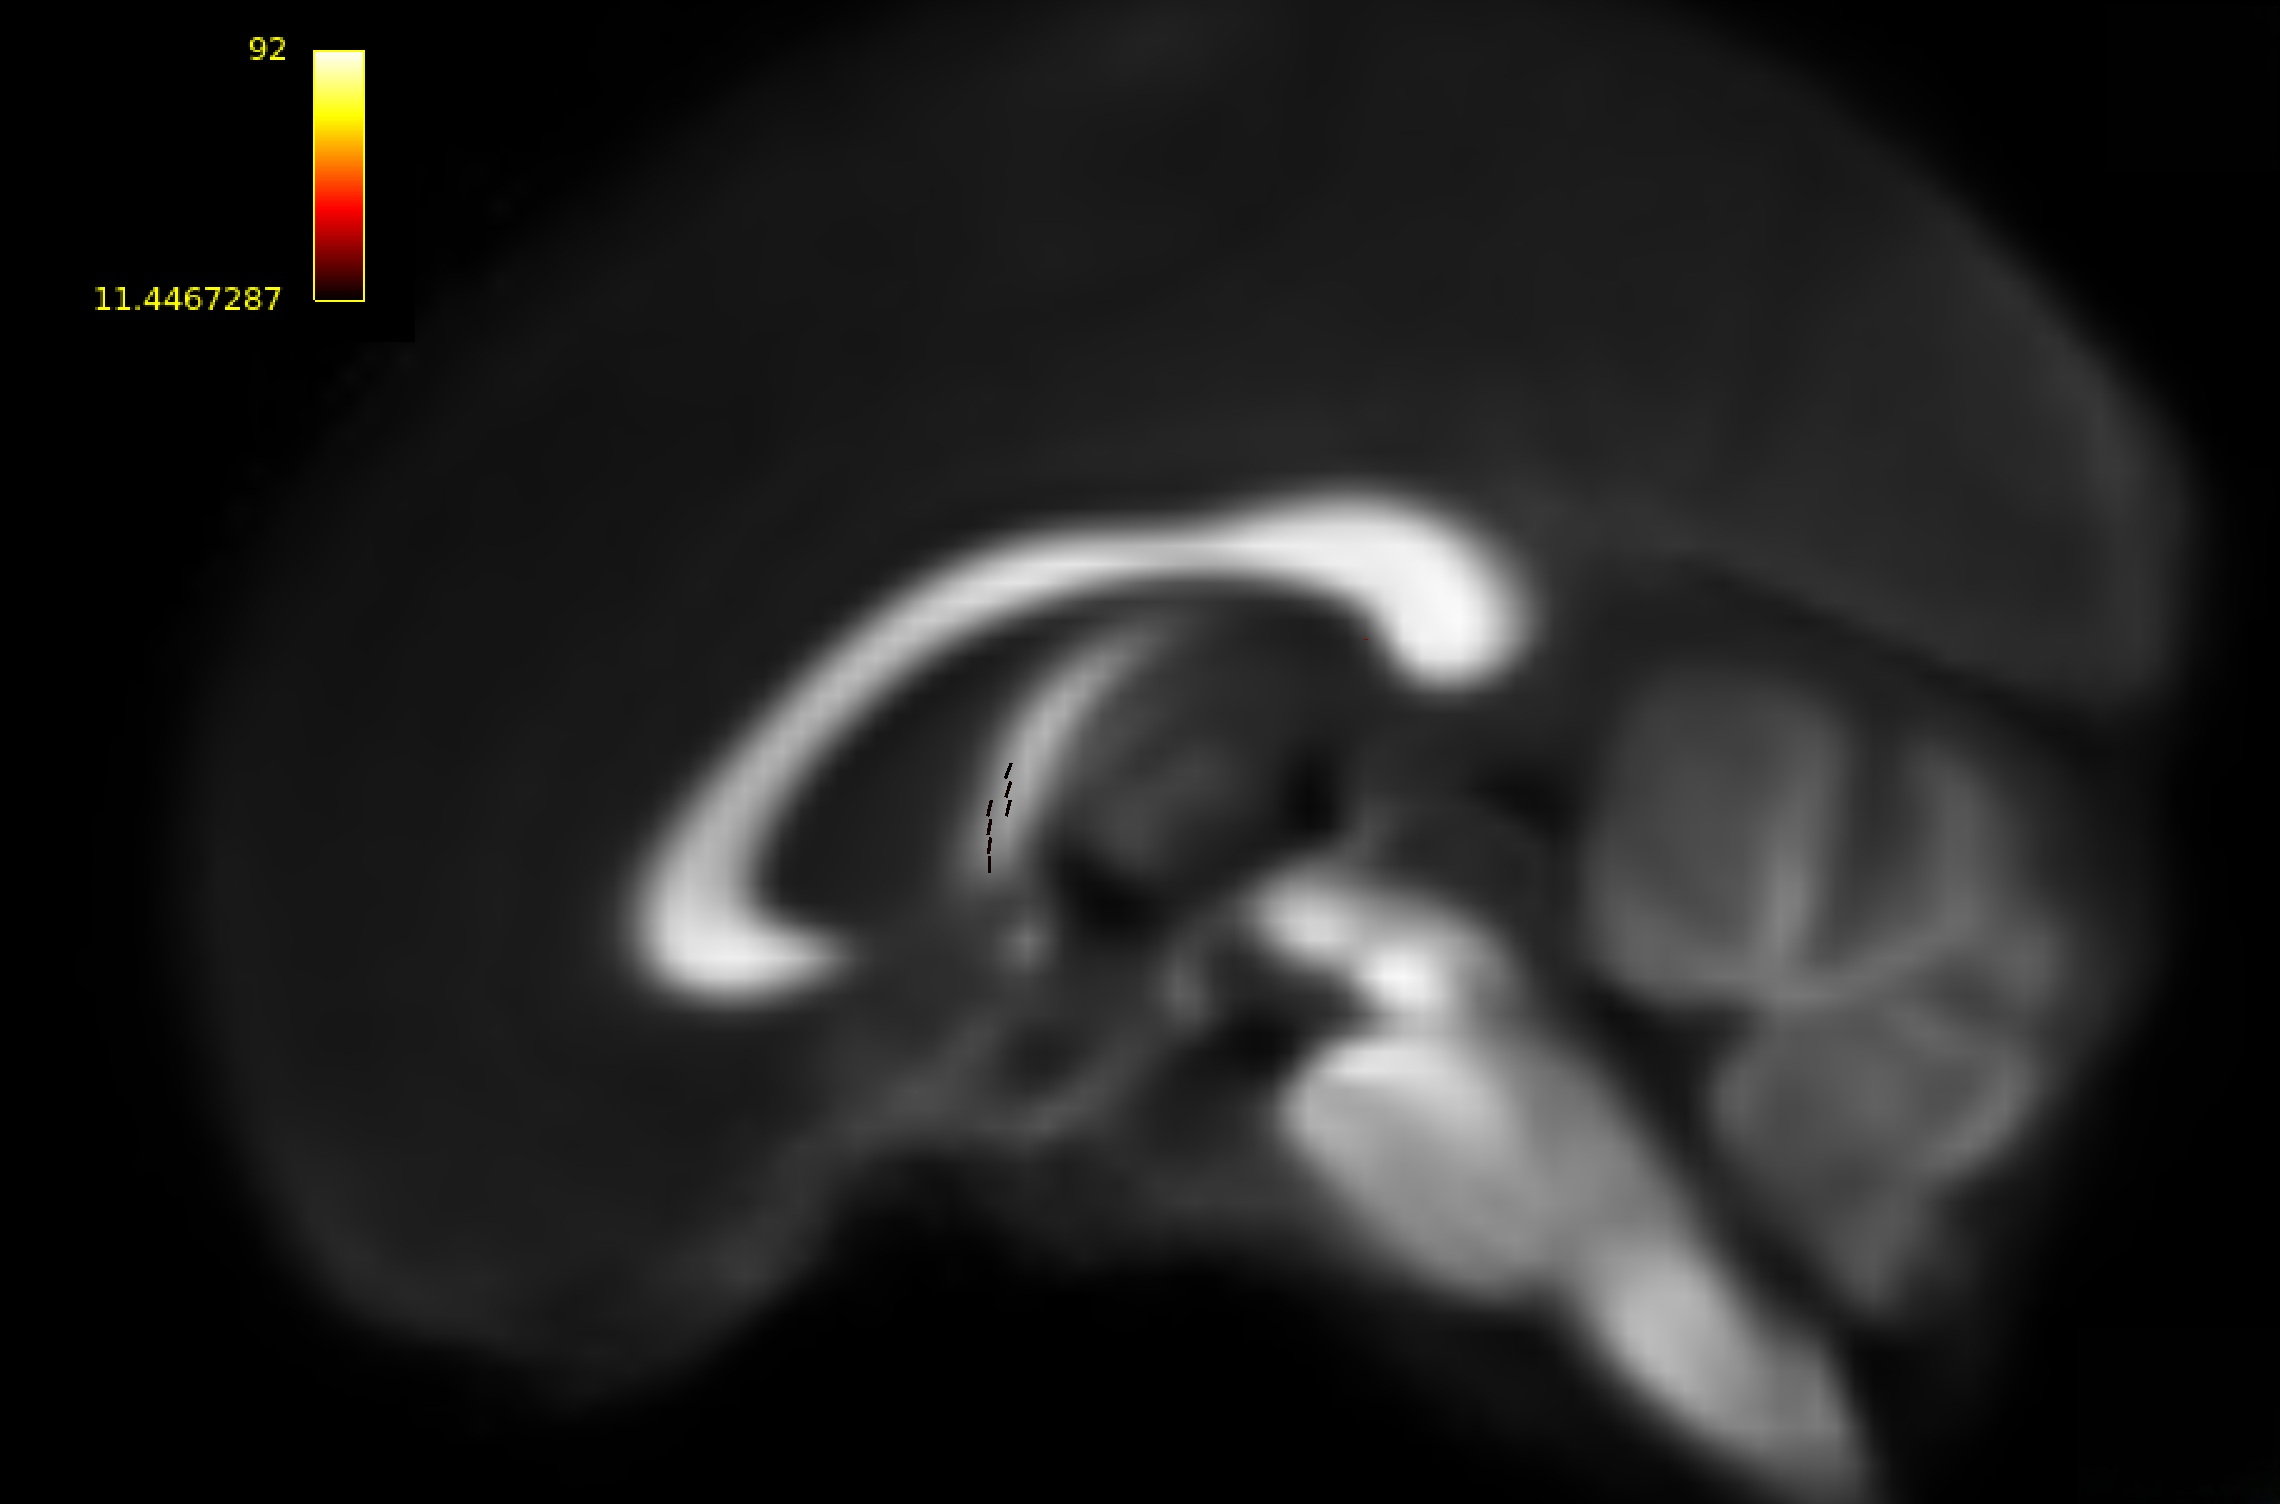
\includegraphics[width=0.45\linewidth]{Images/new_wm0000.jpg}
        \label{fig:subfig-sagittal}
    }
    \hfill
    \subfloat[Coronal view.]{
        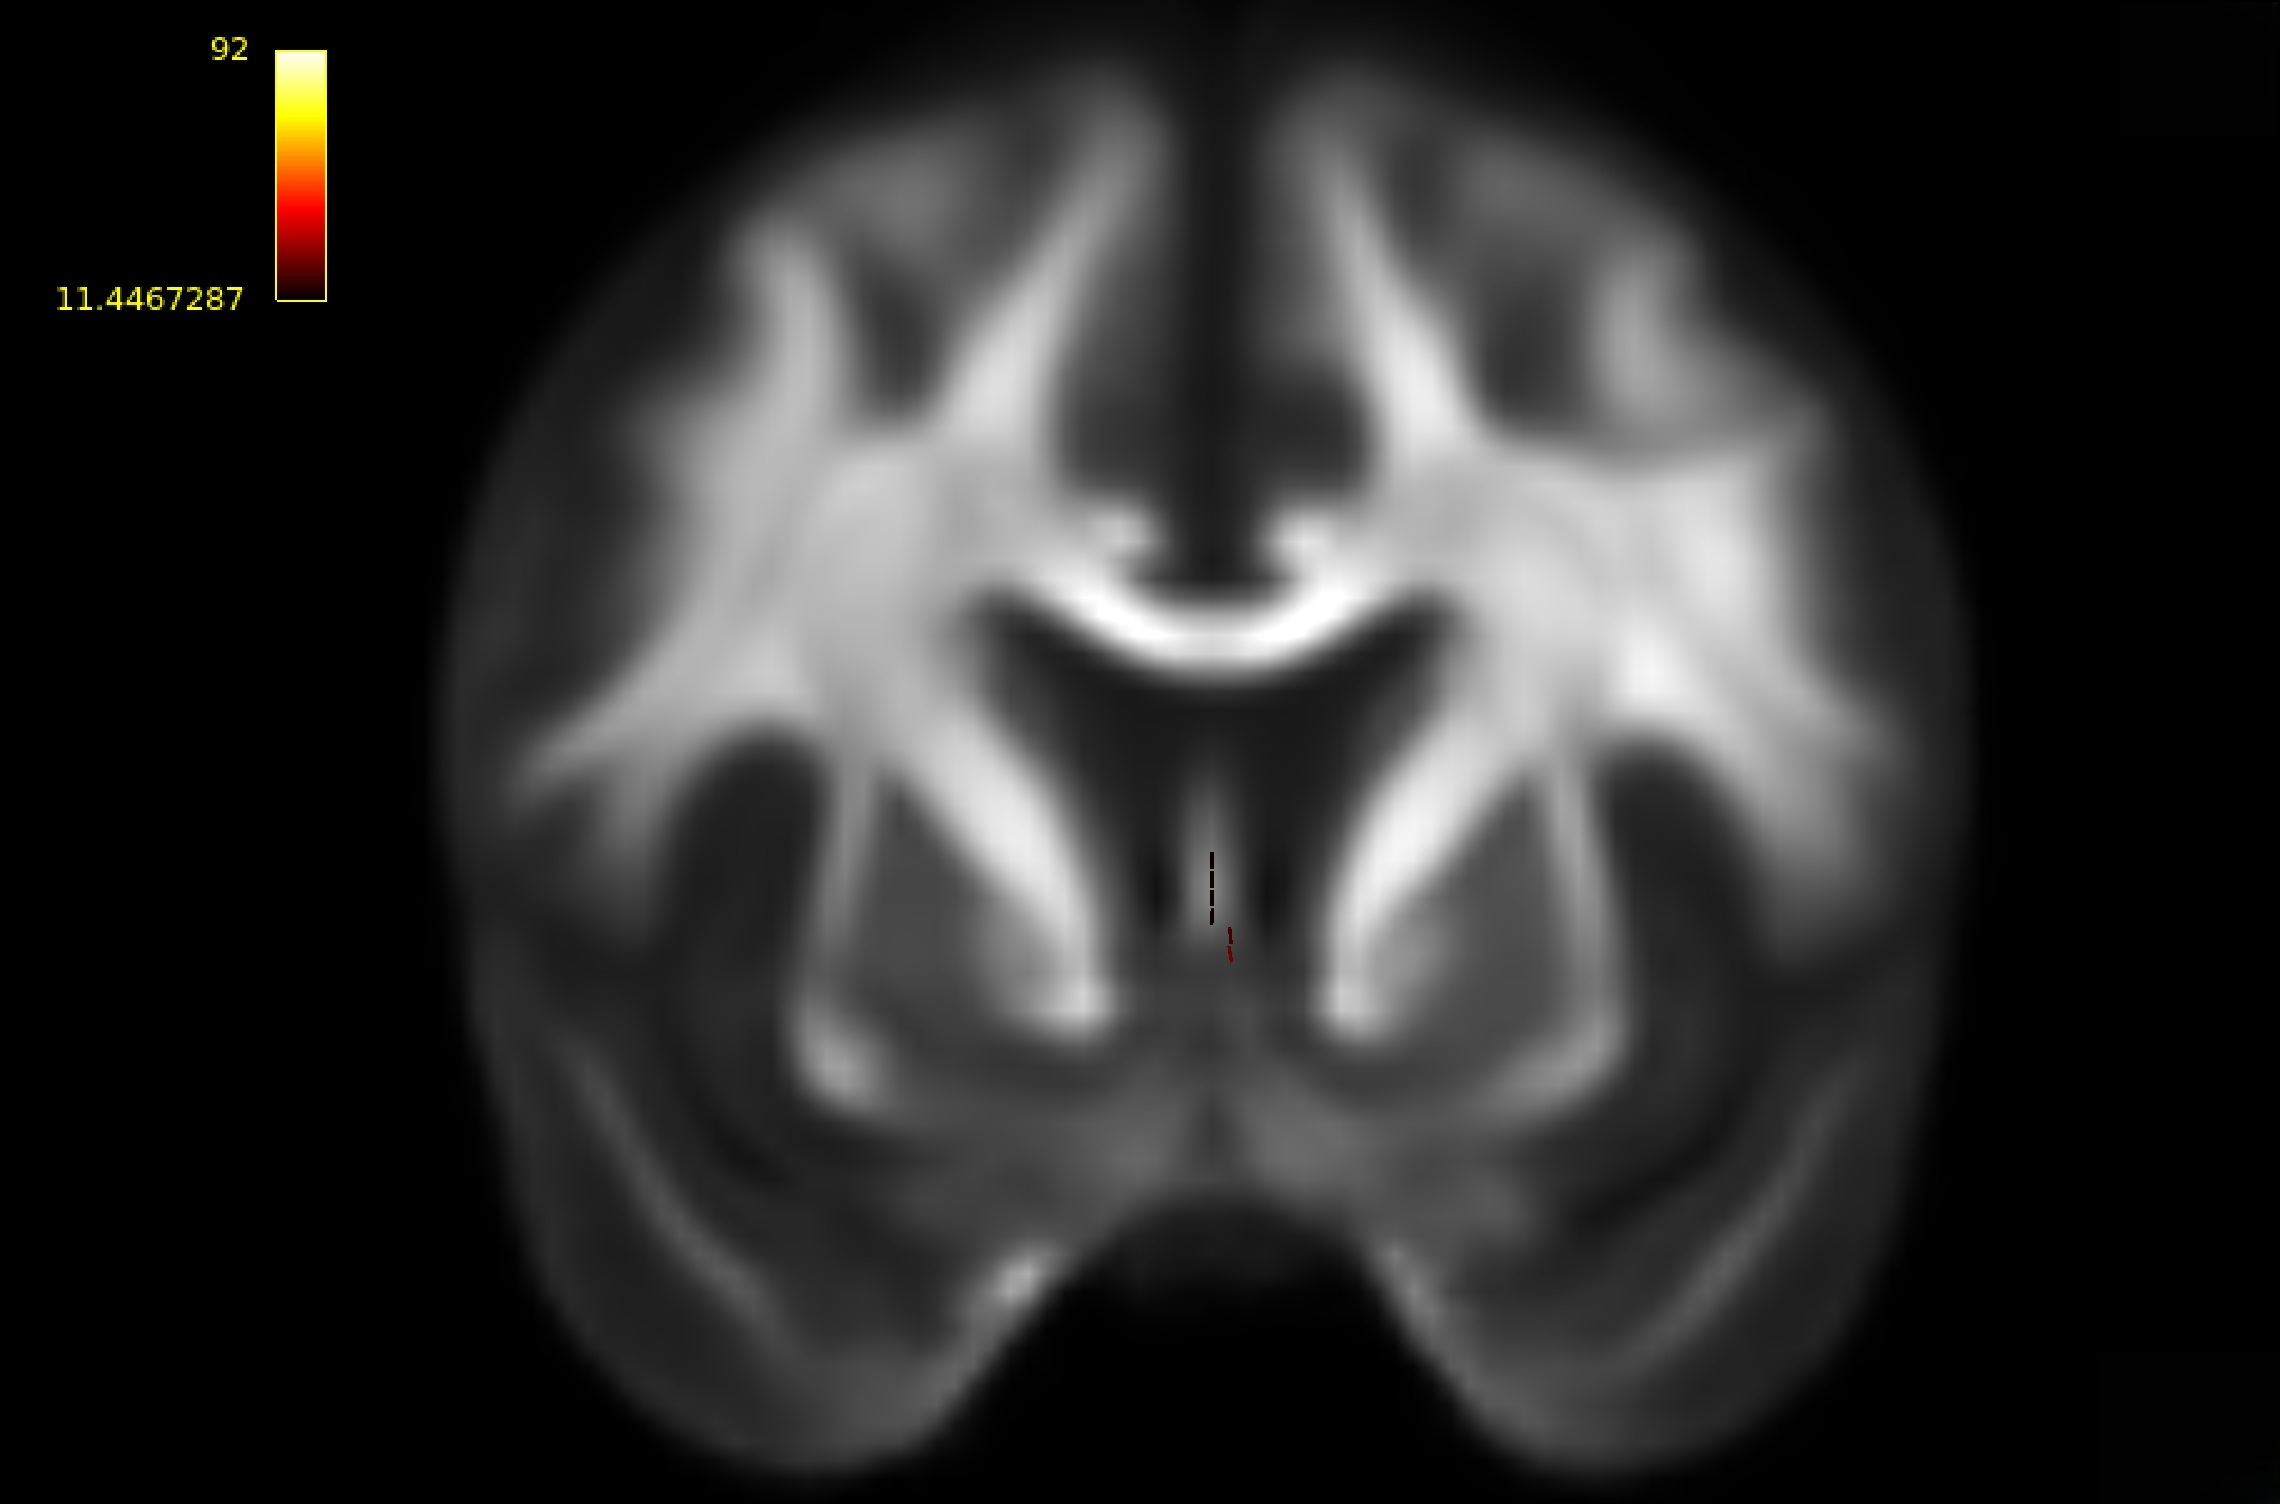
\includegraphics[width=0.45\linewidth]{Images/new_wm0001.jpg}
        \label{fig:subfig-coronal}
    }
    \caption{Fixels extracted from LoRE-SD scaled with the WM contrast, testing for higher AFD in CP compared to HC. The background image is the average WM contrast across all subjects in template space. Only significant fixels are shown, with color indicating the percentage increase relative to HC. Fixels belong to the fornix.}
    \label{fig:fornix4}
\end{figure}



\begin{figure}[h]
  \centering
  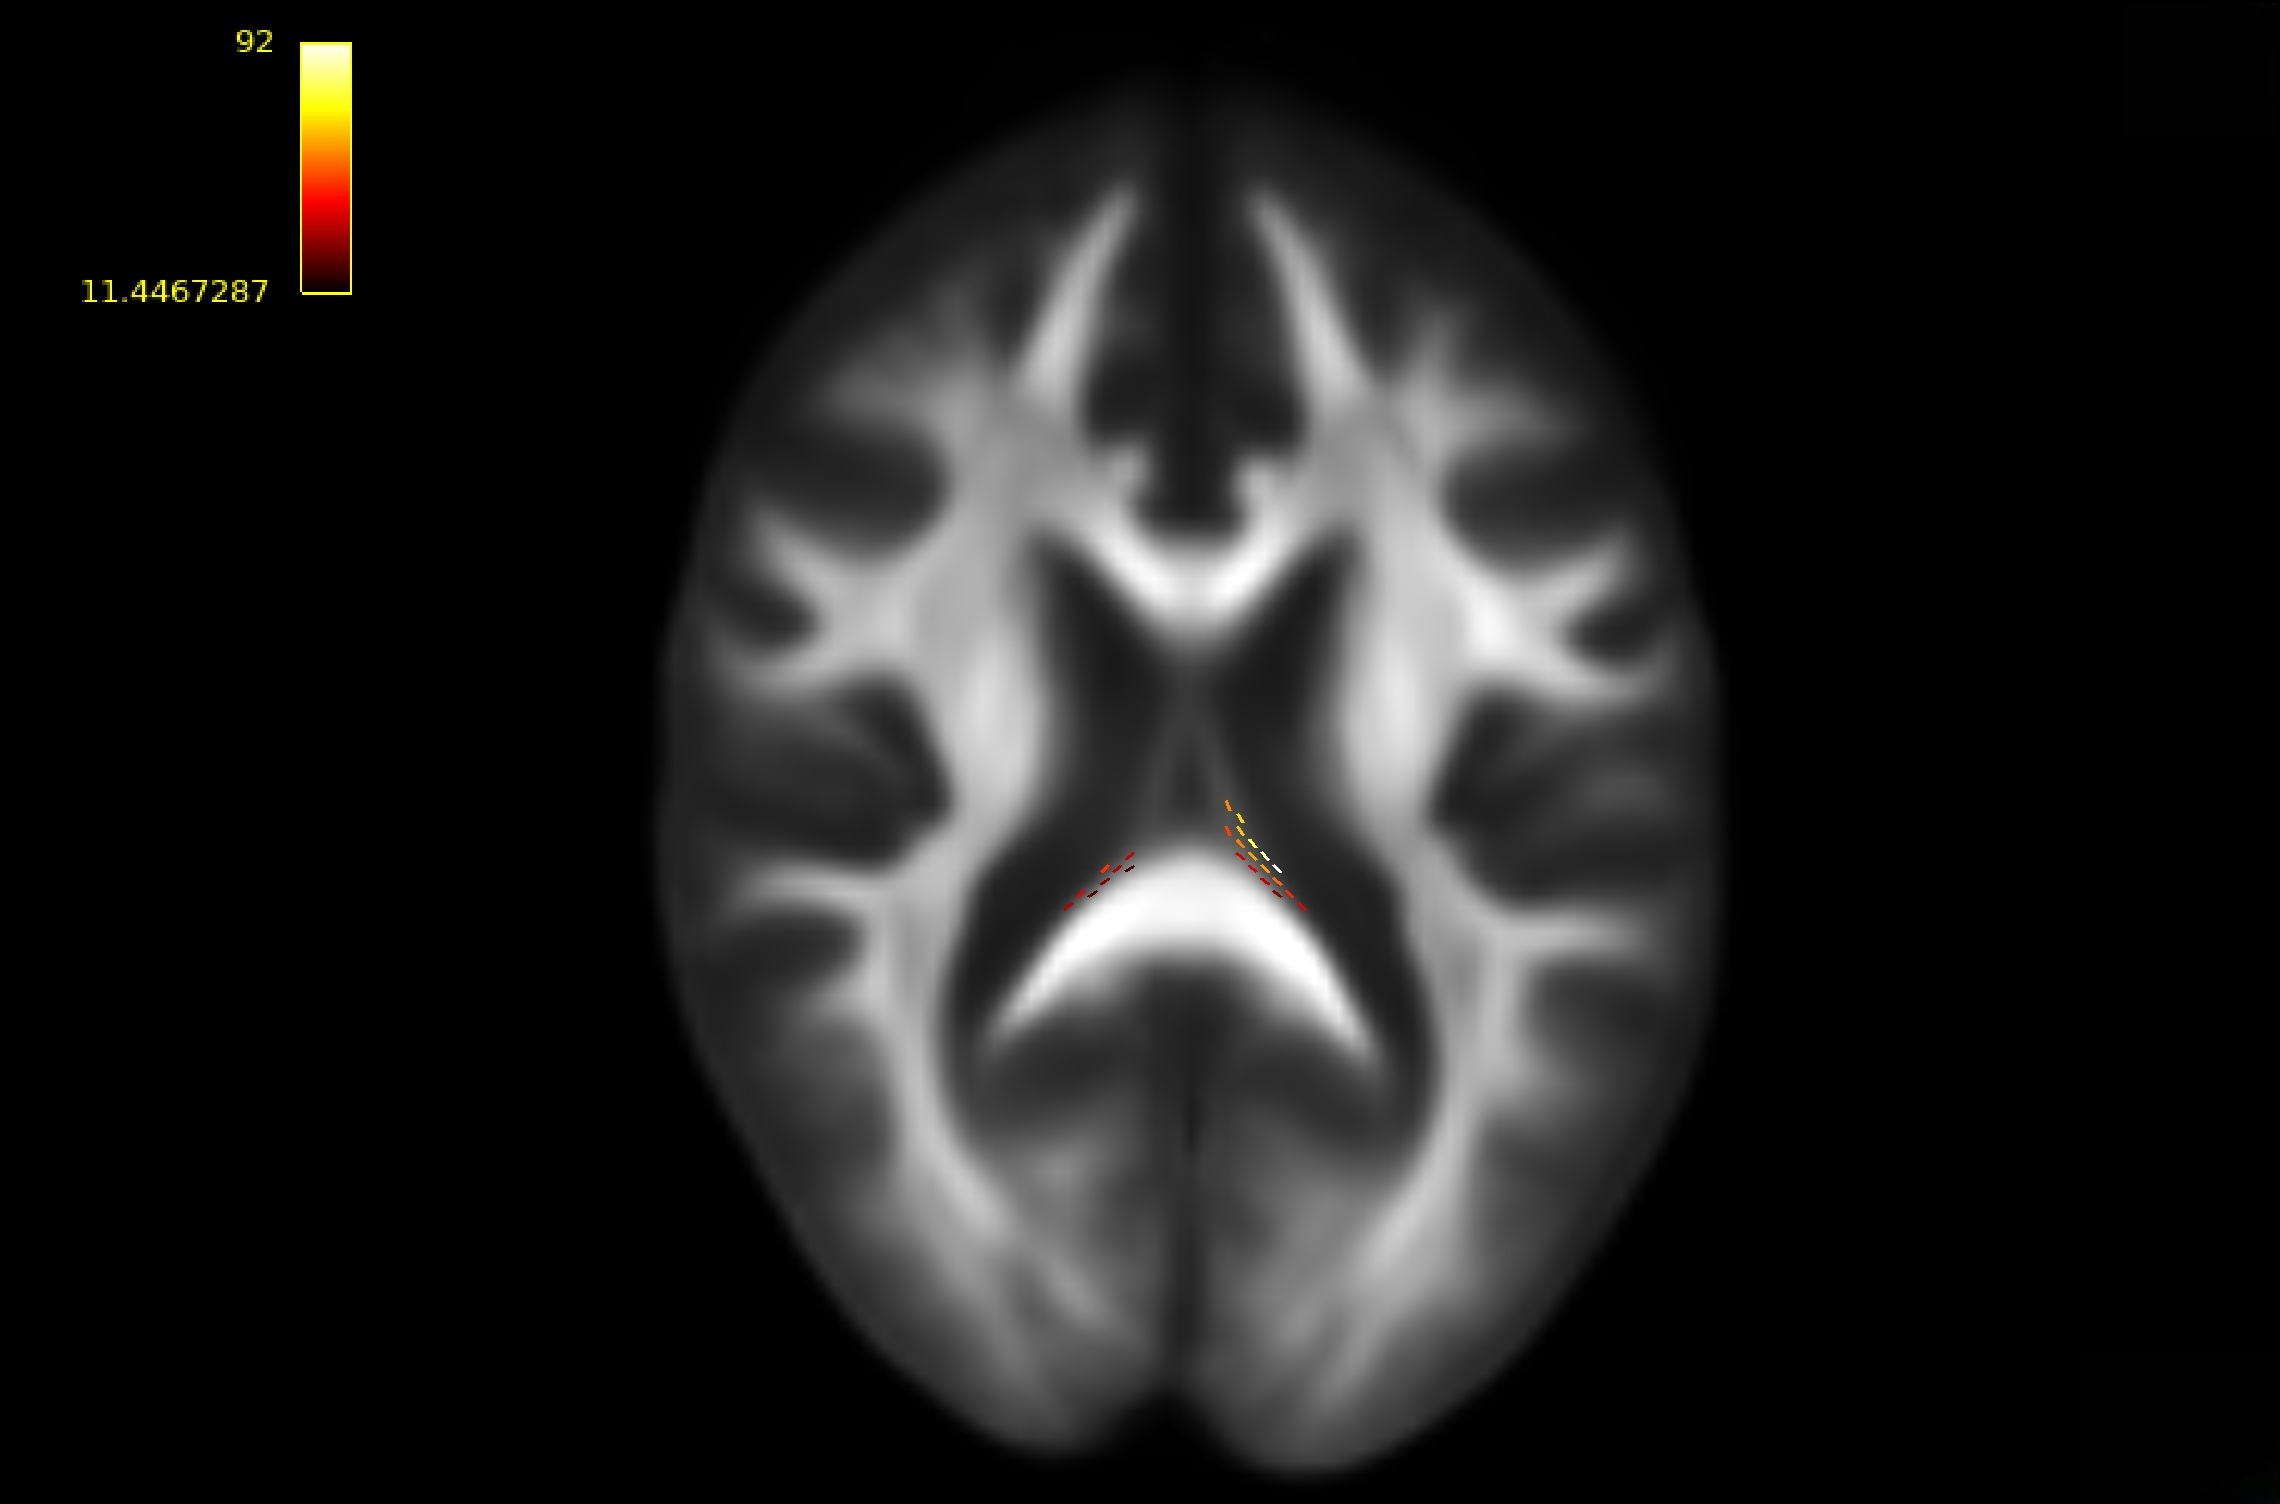
\includegraphics[width=0.9\textwidth]{Images/new_wm0002.jpg} % or use height= for vertical sizing
  \caption{LoRE-SD scaled with the WM contrast, testing for higher AFD in CP compared to HC. Only significant fixels are shown and the color represents the percentage increase relative to HC. The image in the background is the average WM contrast across all subjects in template space. Fixels are part of the fornix, corpus callosum and interface with the ventricles.}
  \label{fig:wm_result}
\end{figure}

\subsection{Results with reduced fixel mask}
To reduce the number of fixels and increase statistical power, a threshold was applied to include only fixels with a sufficient number of streamlines passing through them, before repeating the analysis. For MT-CSD ODFs, a threshold of 250 streamlines was used. This reduced the total number of fixels in the analysis mask from 287,483 (after excluding the cerebellum and brainstem) to 157,821, while preserving overall WM connectivity, as no major fibre bundles were excluded. Figure~\ref{fig:reduced} illustrates the fixels excluded by this thresholding process, which were predominantly located in regions of complex fibre crossings and at tissue boundaries.

\begin{figure}[h]
    \centering
    \subfloat[Sagittal view]{
        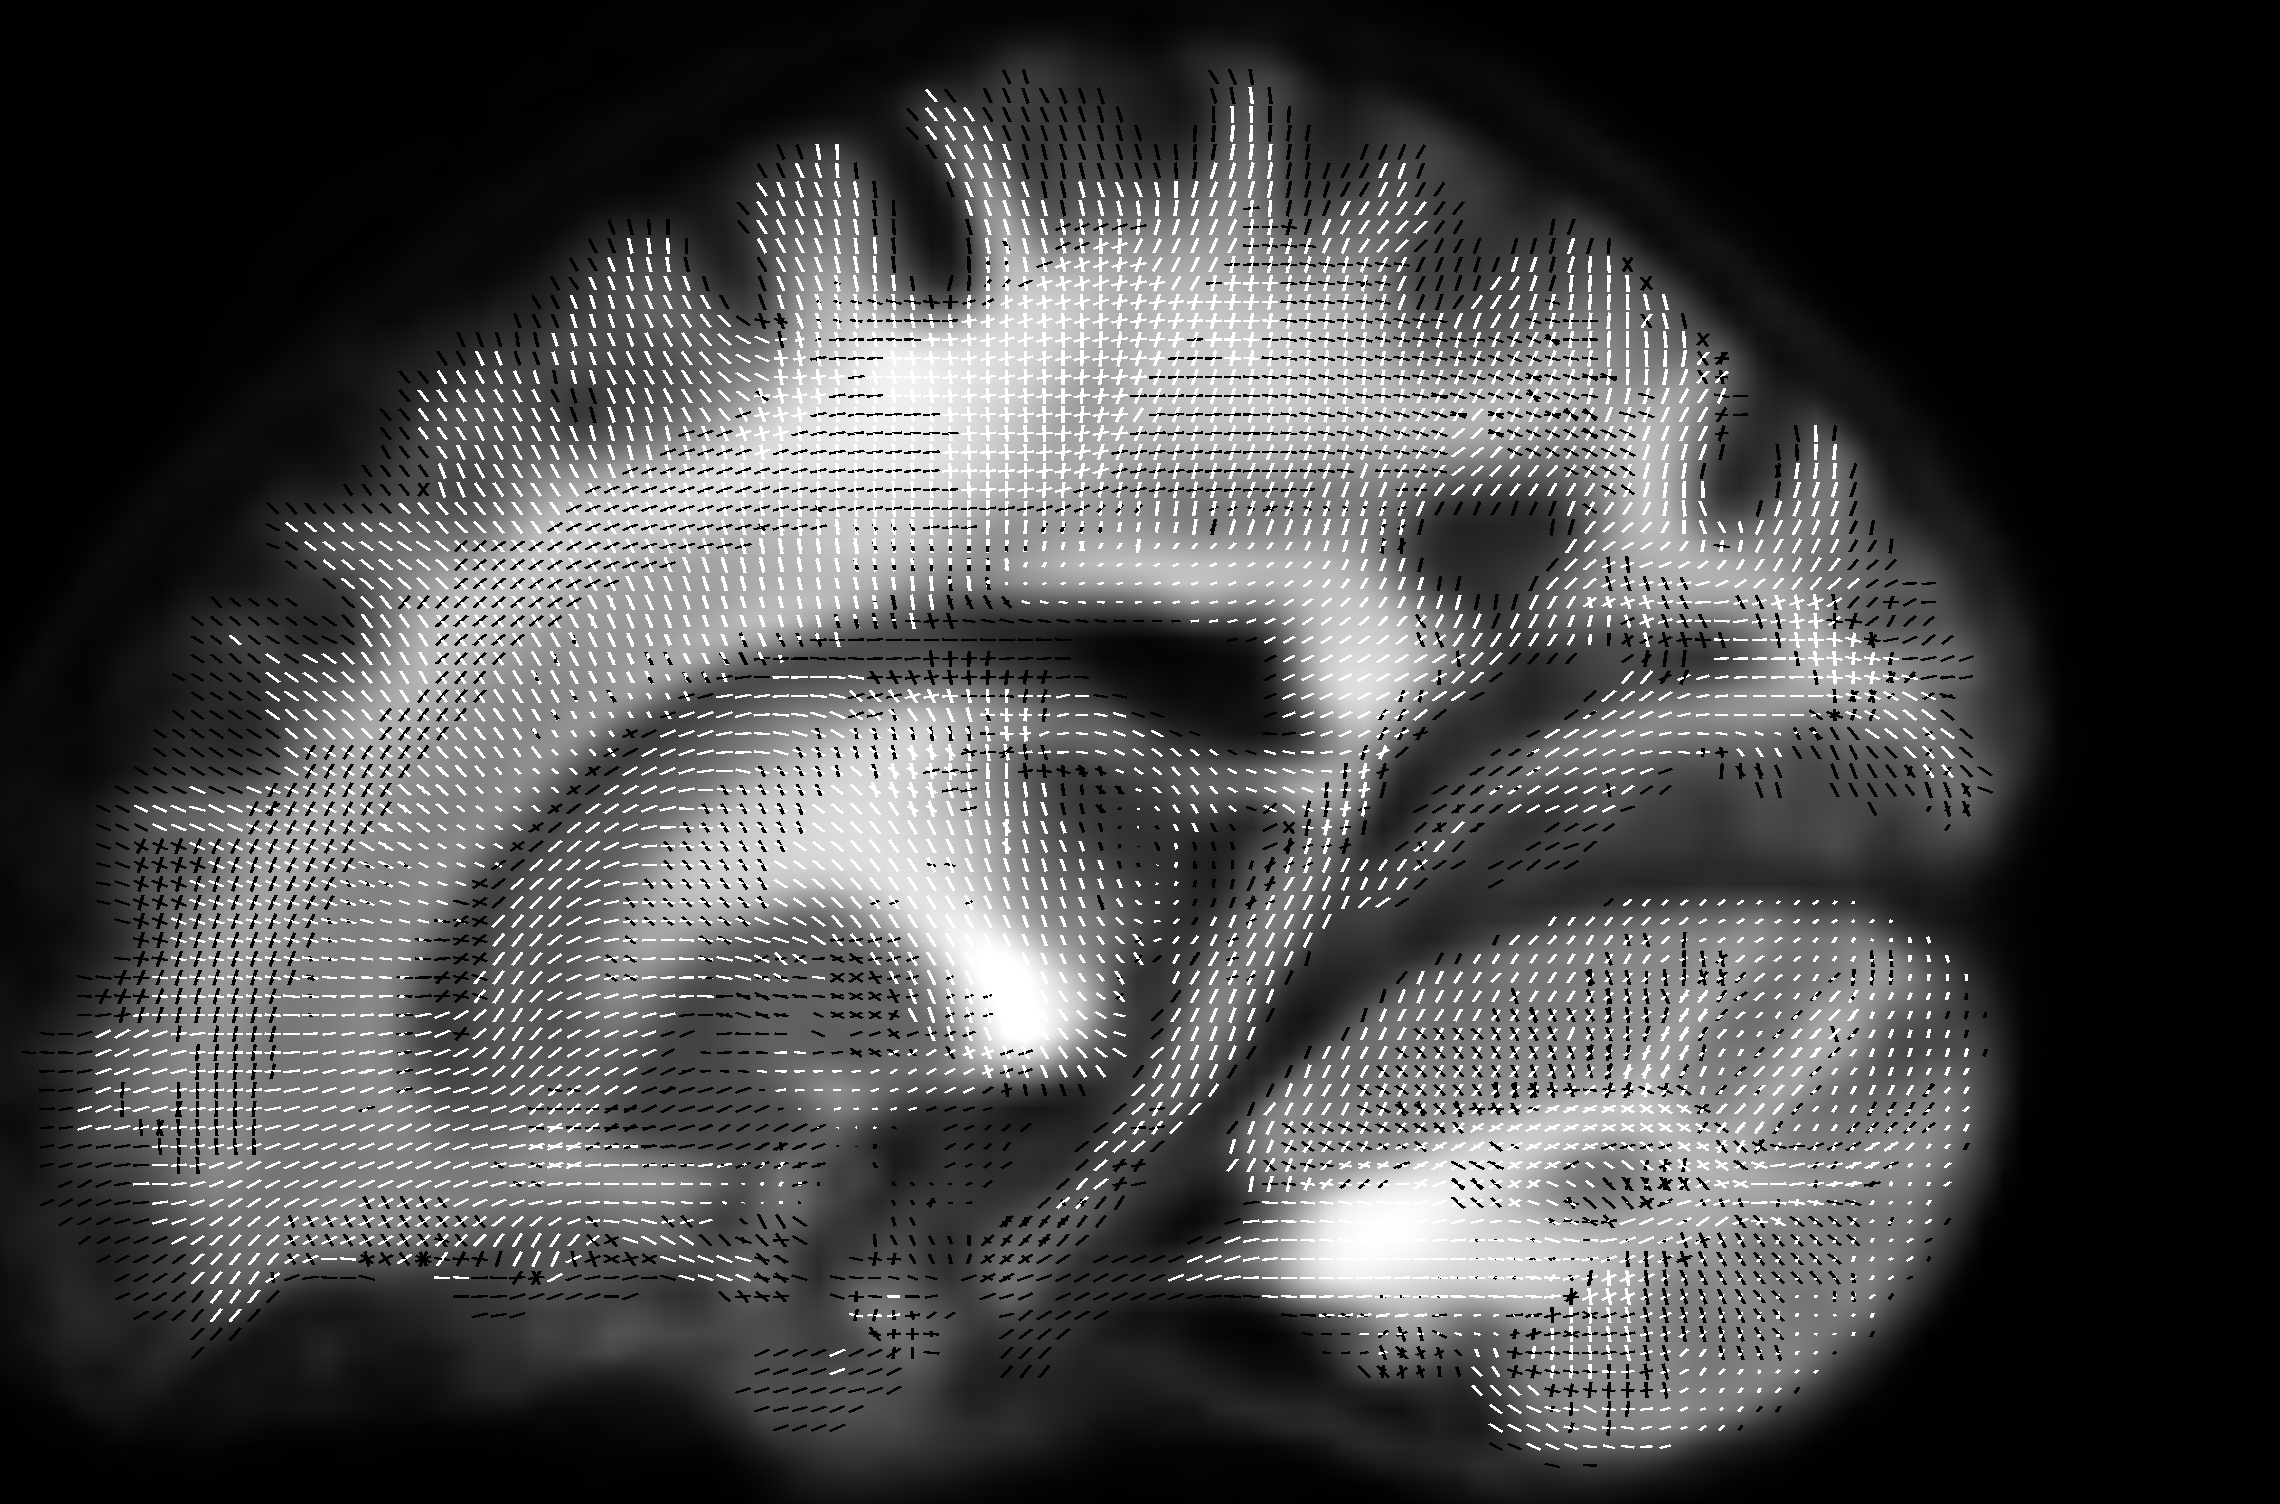
\includegraphics[width=0.5\linewidth]{Images/250_mask_MT0000.jpg}
        \label{fig:subfig-sagittal-mask}
    }
    \hfill
    \subfloat[Coronal view]{
        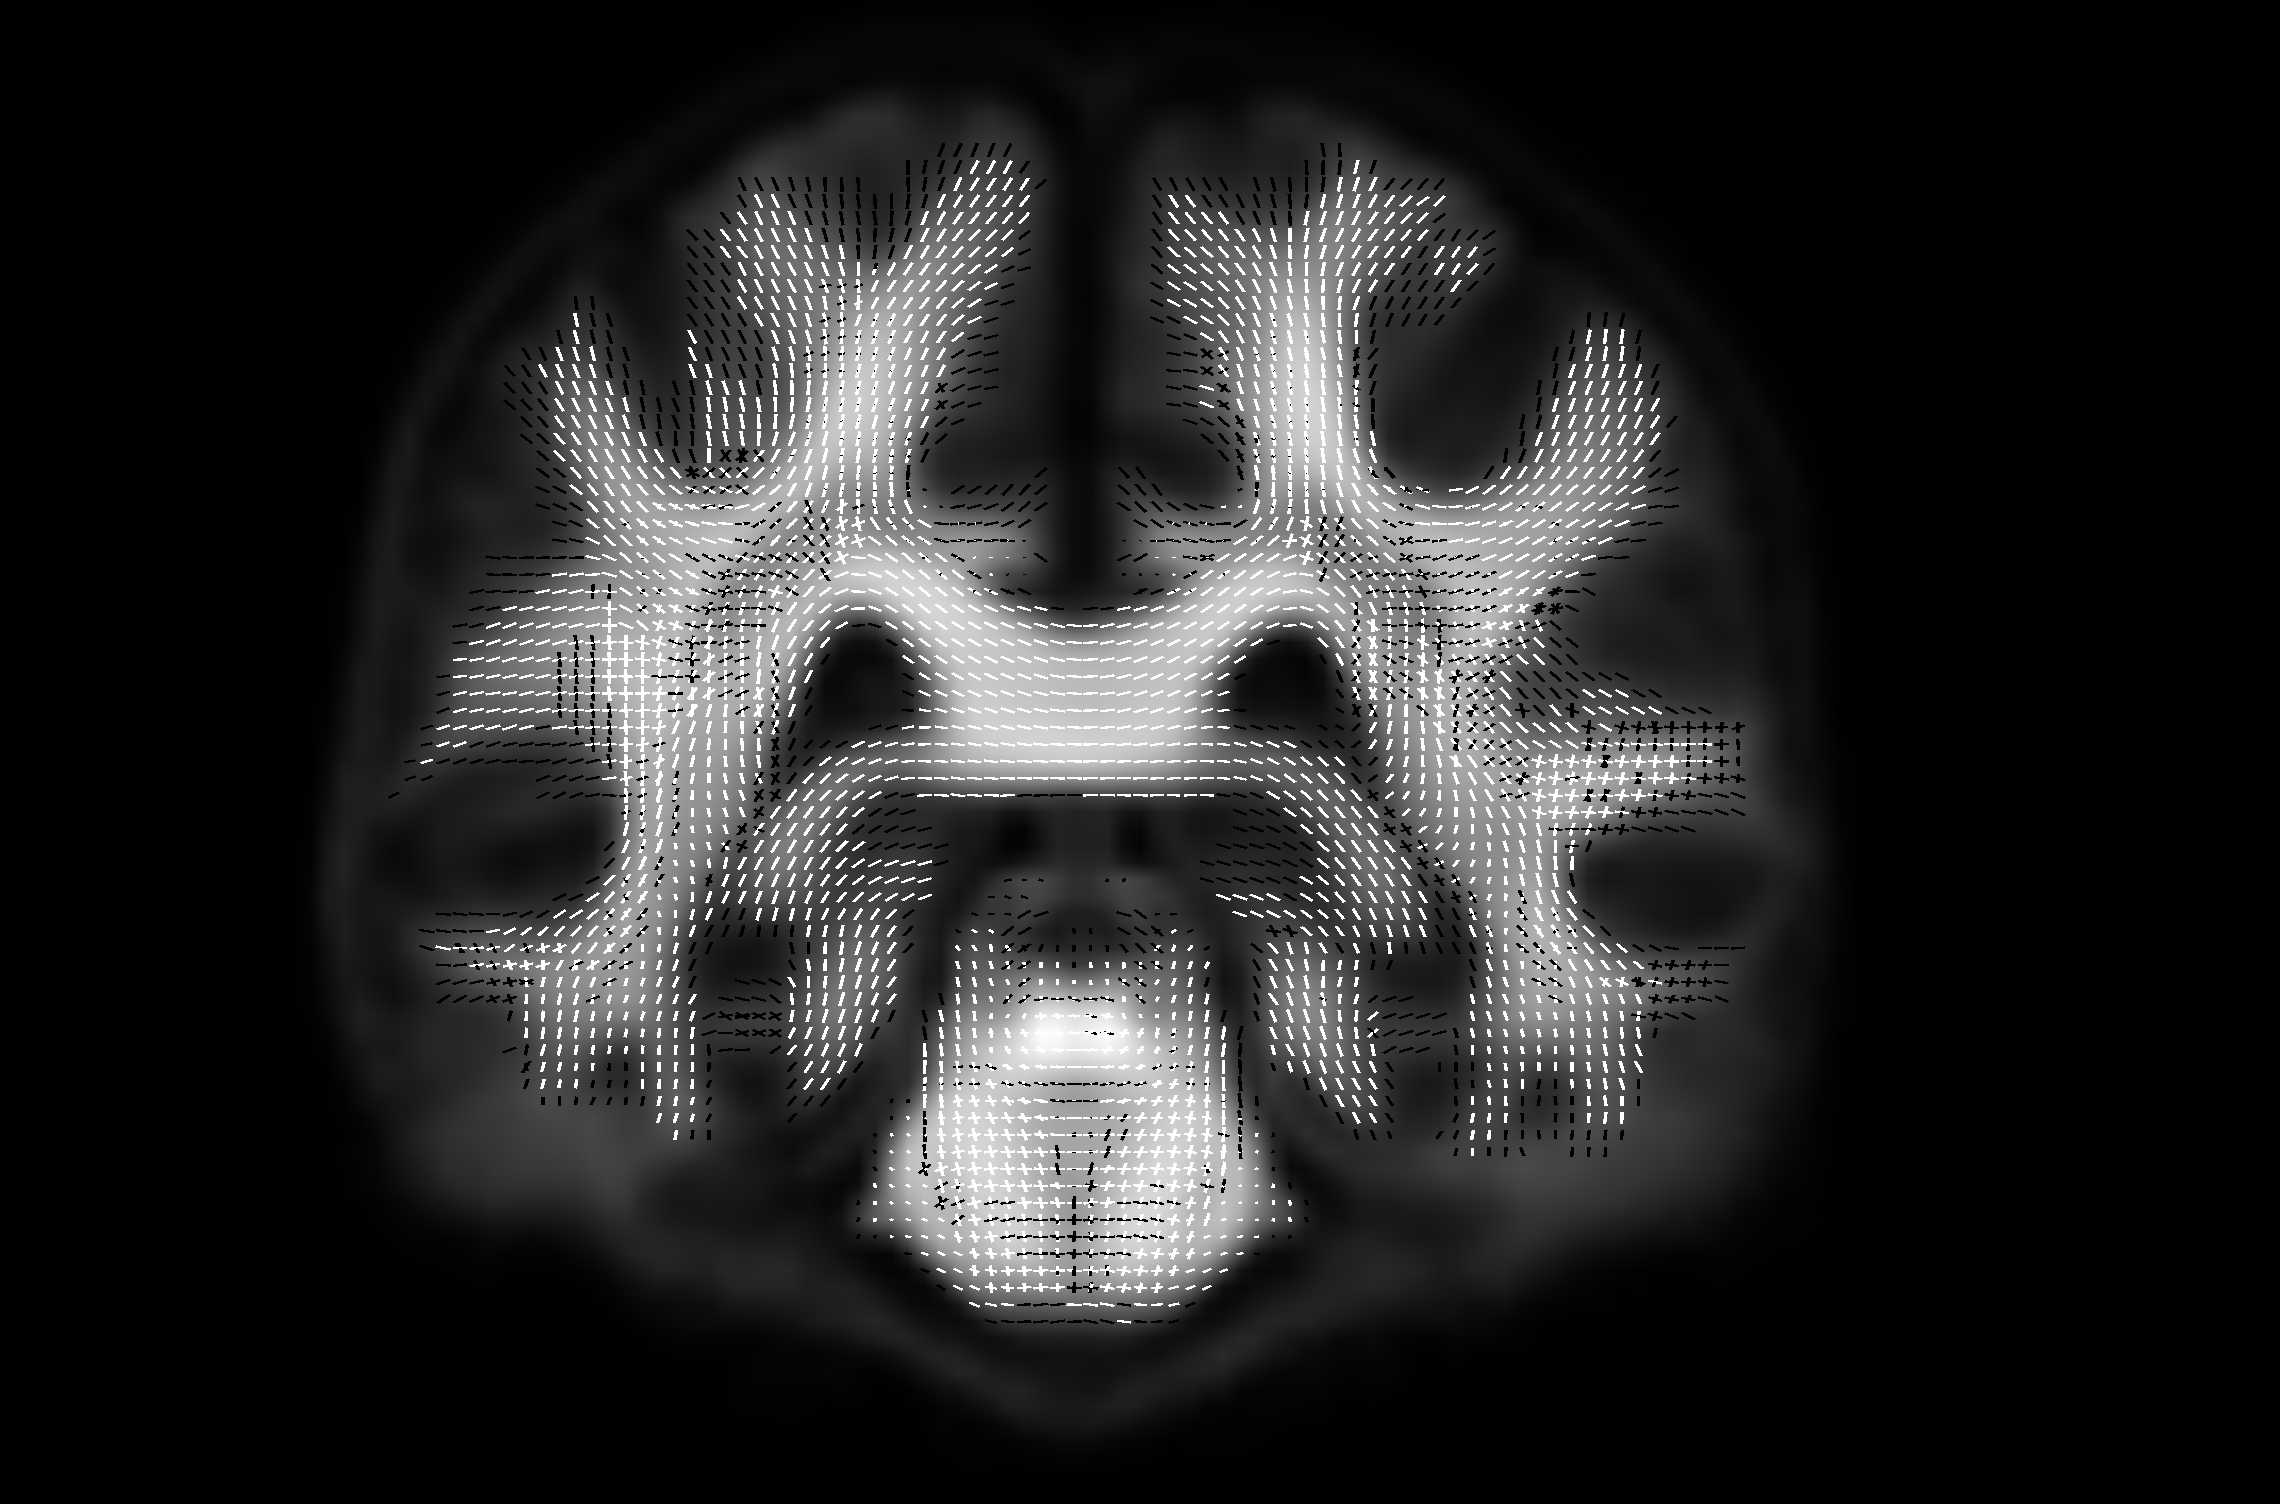
\includegraphics[width=0.5\linewidth]{Images/250_mask_MT0009.jpg}
        \label{fig:subfig-coronal-mask}
    }
    \caption{Reduced fixel mask for the MT-CSD-derived template after applying a threshold on the number of streamlines. Only fixels with more than 250 streamlines passing through them are retained (shown in white); excluded fixels are shown in black.}
    \label{fig:reduced}
\end{figure}


For the AFD metric, after excluding low-density fixels based on streamline count ($\geq$250), we identified 868 fixels showing a significant increase in the CP group compared to HC. No other contrasts gave significant results for AFD. Examples of these findings are presented in Figure~\ref{fig:reduced_MT}. Notably, the maximum effect size decreased with the reduced mask, and fewer significant fixels were detected at tissue interfaces, likely due to the exclusion of possible spurious fibres in these regions. In contrast, there was a relative increase in significant fixels within the CC.

\begin{figure}[H]
    \centering
    \subfloat[Reduced Fixel Mask]{
        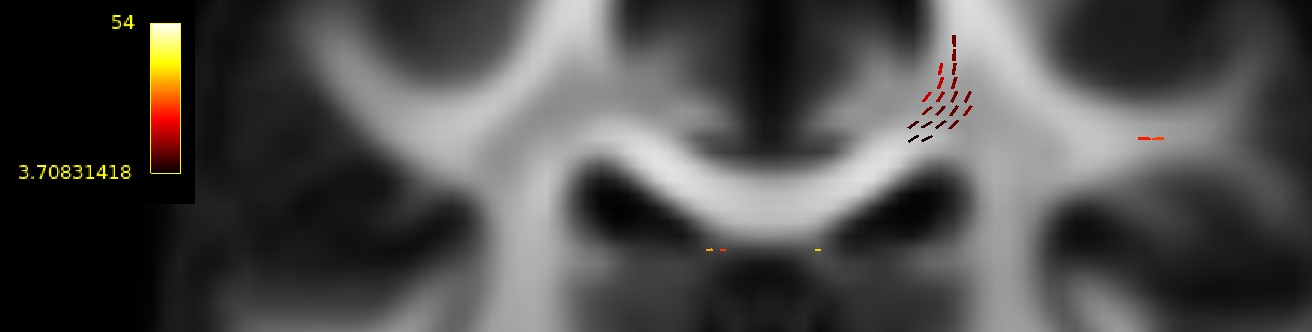
\includegraphics[width=0.8\linewidth]{Images/comp_TDI1.jpg}
        \label{fig:subfig-reduced-fixel}
    } \\[1em] % line break + vertical space
    \subfloat[Full Mask]{
        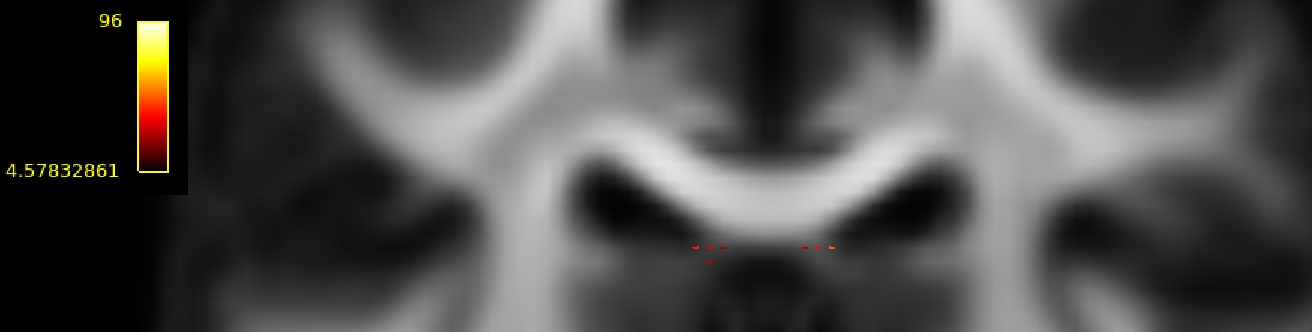
\includegraphics[width=0.8\linewidth]{Images/comp_TDI2.jpg}
        \label{fig:subfig-full-fixel}
    }
    \caption{Fixels extracted with MT-CSD, testing for an increase in AFD in the CP group compared to HC. Significant fixels are shown and colored by percentage increase relative to the mean value in the HC group. (a) Results after reducing the number of fixels by excluding low-density fixels. (b) Original results. Reducing the number of fixels increases statistical power, revealing additional effects, particularly near the CC.}
    \label{fig:reduced_MT}
\end{figure}


For LoRE-SD ODFs scaled with the intra-axonal contrast, applying the streamline threshold (250) reduced the total number of fixels from 320,964 to 196,217. In this case, 66 fixels were found significant for AFD when testing for increased values in CP vs. HC. These included new fixels in the fornix and CC as shown in Figure~\ref{fig:reduced_intra}. Furthermore, additional significant fixels emerged within regions previously identified in the analysis with the full fixel mask.

\begin{figure}[H]
    \centering
    \subfloat[]{
        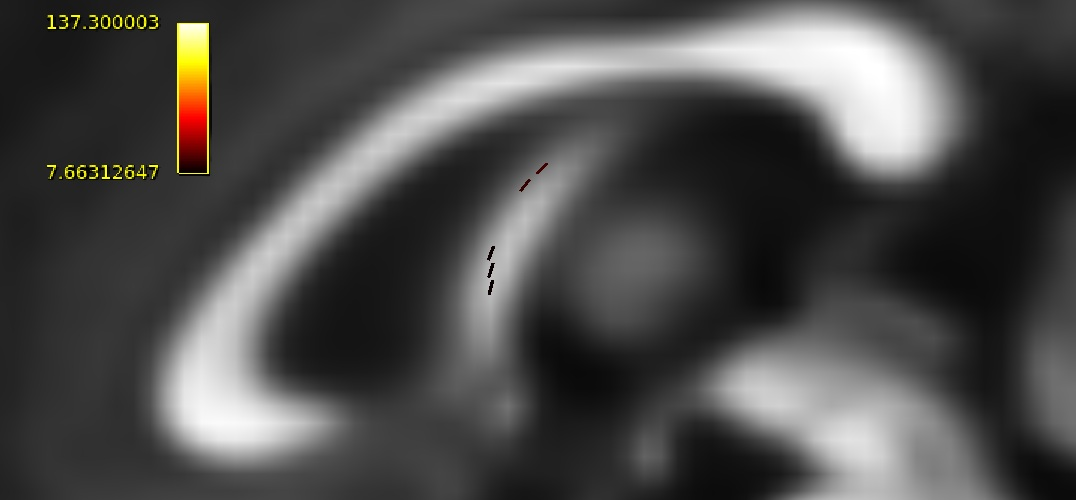
\includegraphics[width=0.5\linewidth]{Images/intra_TDI1.jpg}
        \label{fig:subfig-intra-A}
    }
    \hfill
    \subfloat[]{
        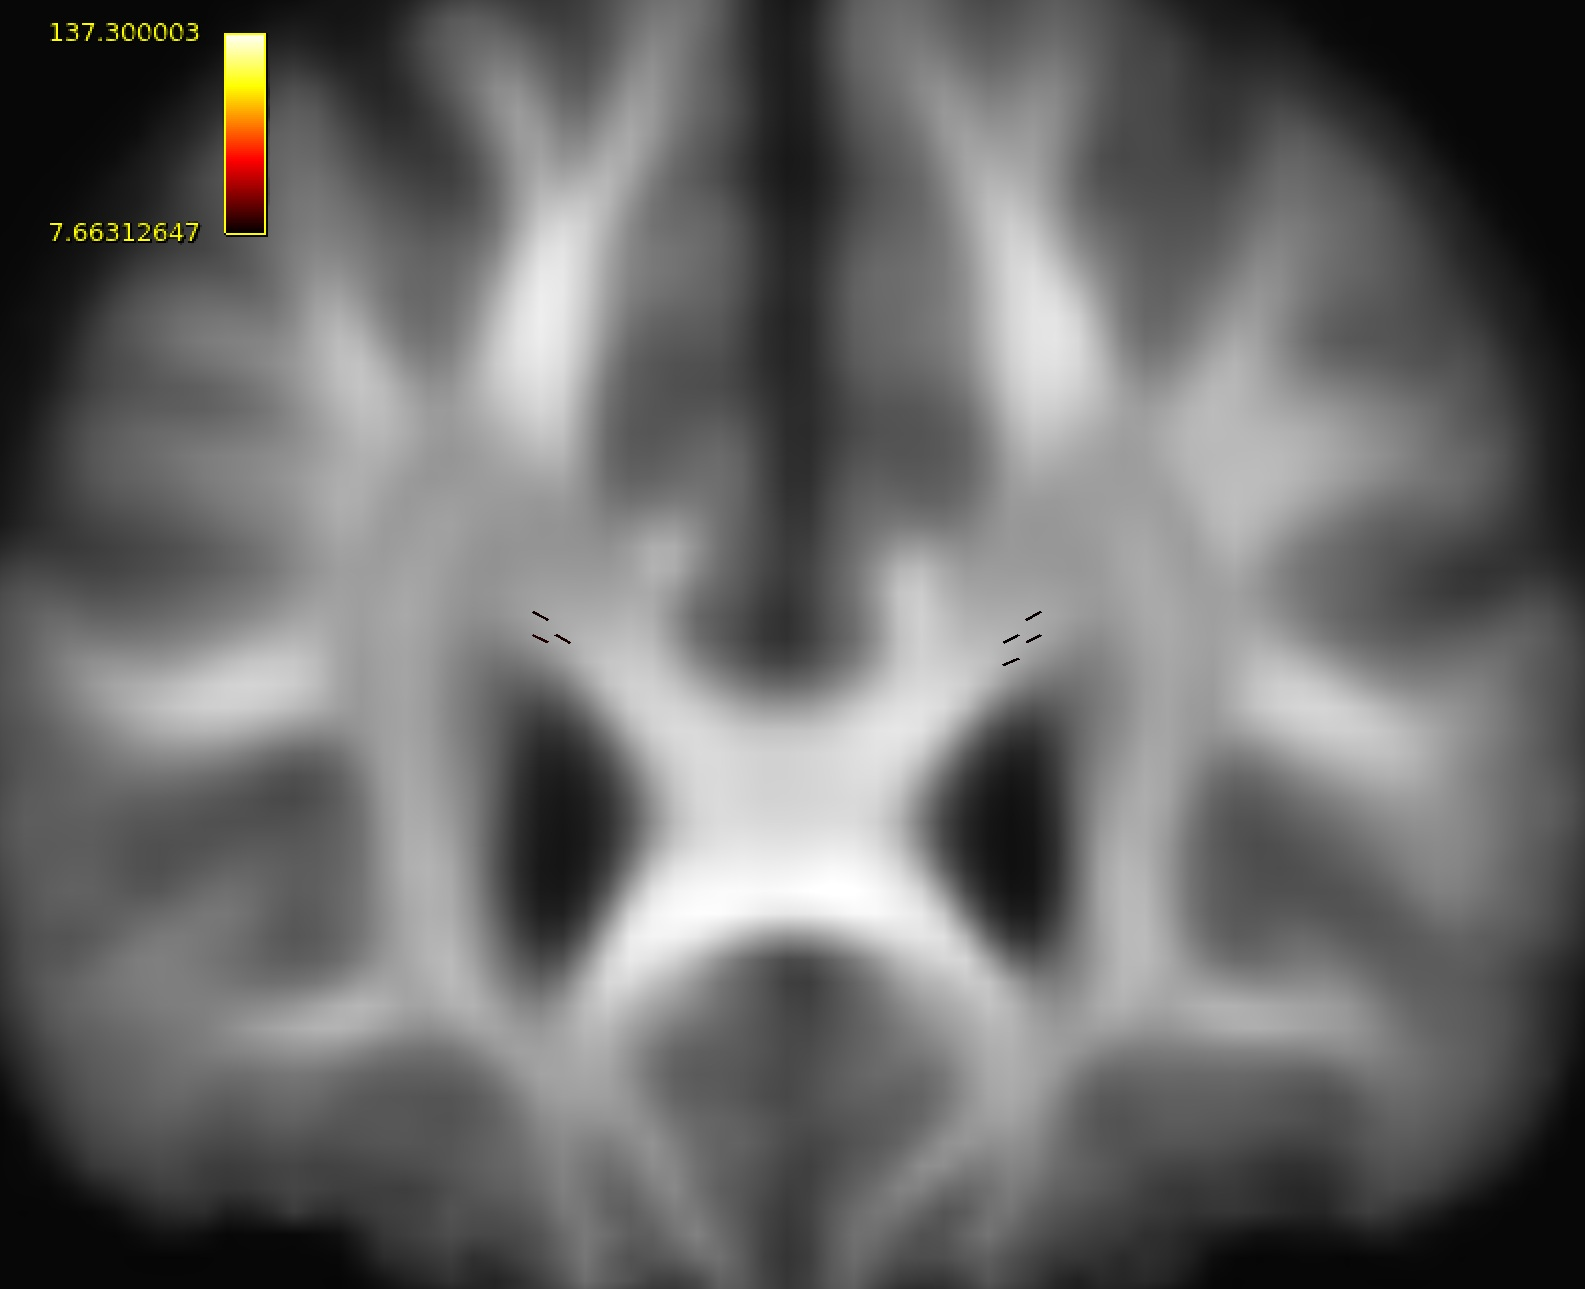
\includegraphics[width=0.5\linewidth]{Images/intra_TDI2.jpg}
        \label{fig:subfig-intra-B}
    }
    \caption{Fixels extracted from LoRE-SD scaled with the intra-axonal contrast, testing for higher AFD in CP compared to HC using the reduced fixel mask. Compared to the full mask results, new significant fixels are detected in the fornix (a) and near the genu of the corpus callosum (b). Only significant fixels are shown, colored by percentage increase relative to HC.}
    \label{fig:reduced_intra}
\end{figure}


With the FA scaling contrast, no significant fixels were detected even after applying the reduced fixel mask.
However, using the WM contrast, 162 fixels showed a significant increase in AFD in the CP group compared to HC. These fixels were in the regions identified in the original analysis.


